\documentclass[10pt,letterpaper]{article}
\usepackage[top=1in,bottom=1in,left=1in,right=1in]{geometry}
\usepackage{datetime}
\usepackage{natbib}      % http://merkel.zoneo.net/Latex/natbib.php
\usepackage{palatino}
\usepackage{verbatim}
\usepackage[normalem]{ulem}
\bibpunct{(}{)}{;}{a}{,}{,}

\usepackage{array}

\usepackage{chngpage}
\usepackage{stmaryrd}
\usepackage{amssymb}
\usepackage{amsmath}
\usepackage{graphicx}
\usepackage{lscape}
\usepackage{subfigure}
\usepackage[usenames,dvipsnames]{color}
\definecolor{myblue}{rgb}{0,0.1,0.6}
\definecolor{mygreen}{rgb}{0,0.3,0.1}
\usepackage[colorlinks=true,linkcolor=black,citecolor=mygreen,urlcolor=myblue]{hyperref}

\newcommand{\bocomment}[1]{\textcolor{Bittersweet}{BO says: #1}}

\newcommand{\ignore}[1]{}
\newcommand{\transpose}{^\mathsf{T}}
\newcommand{\inner}[1]{\langle #1 \rangle} 
\newcommand{\smallsec}[1]{\noindent \textbf{#1\ }}
\newcommand{\cmd}[1] {{\color{blue}\texttt{#1}}}

\newcommand{\solution}[1]{{\color{myblue} \emph{[Solution:} 
#1 

\emph{End solution]}}}
\newcommand{\solutionnote}[1]{{\color{myblue} \emph{[Note:}

#1 

\emph{End note]}}}
\newcommand{\points}[1]{{\color{mygreen}\emph{[#1]\ \ }}}

\newcommand{\aone}{\diamondsuit}
\newcommand{\atwo}{\heartsuit}
\newcommand{\bone}{\triangle}
\newcommand{\btwo}{\Box}
\newcommand{\myand}{\ \land\ }
\newcommand{\myor}{\ \lor\ }
\newcommand{\mynot}{\lnot}

\title{
  \textbf{Panaromic Stiching} \\
}
\settimeformat{ampmtime}
\date{}
\begin{document}
\maketitle

\renewcommand\thesubsection{\thesection.\alph{subsection}}


RANSAC algorithm to stitch two images. The input to the algorithm are two images which are related by an unknown transformation.  blobs detector is  implemented to extract keypoints and extract feature descriptors on them.  The goal is to estimate an affine transformation using feature matching and RANSAC to produce a combined image. 

the overall steps in the alignment algorithm are:
\begin{enumerate}
\item Detect keypoints in each image (part 1).
\item Extract SIFT features at each detected keypoints.
\item Match features based on pairwise distance.
\item Use RANSAC to estimate the best affine transformation.
\item Stitch the two images using the estimated transformation.
\end{enumerate}


There are few difficult test images where affine transformation will not produce perfect results. There are certain kinds of 2D transformation cannot be modeled as affine (See section 2.1 in \href{http://szeliski.org/Book/drafts/SzeliskiBook_20100903_draft.pdf}{Richard Szeliski's book}). Try to align two images with homography transformation, which is more general than affine, to improve the results.

Below are the results using both affine and homographic transformation to stitch two images

\begin{figure}[h]
\centering
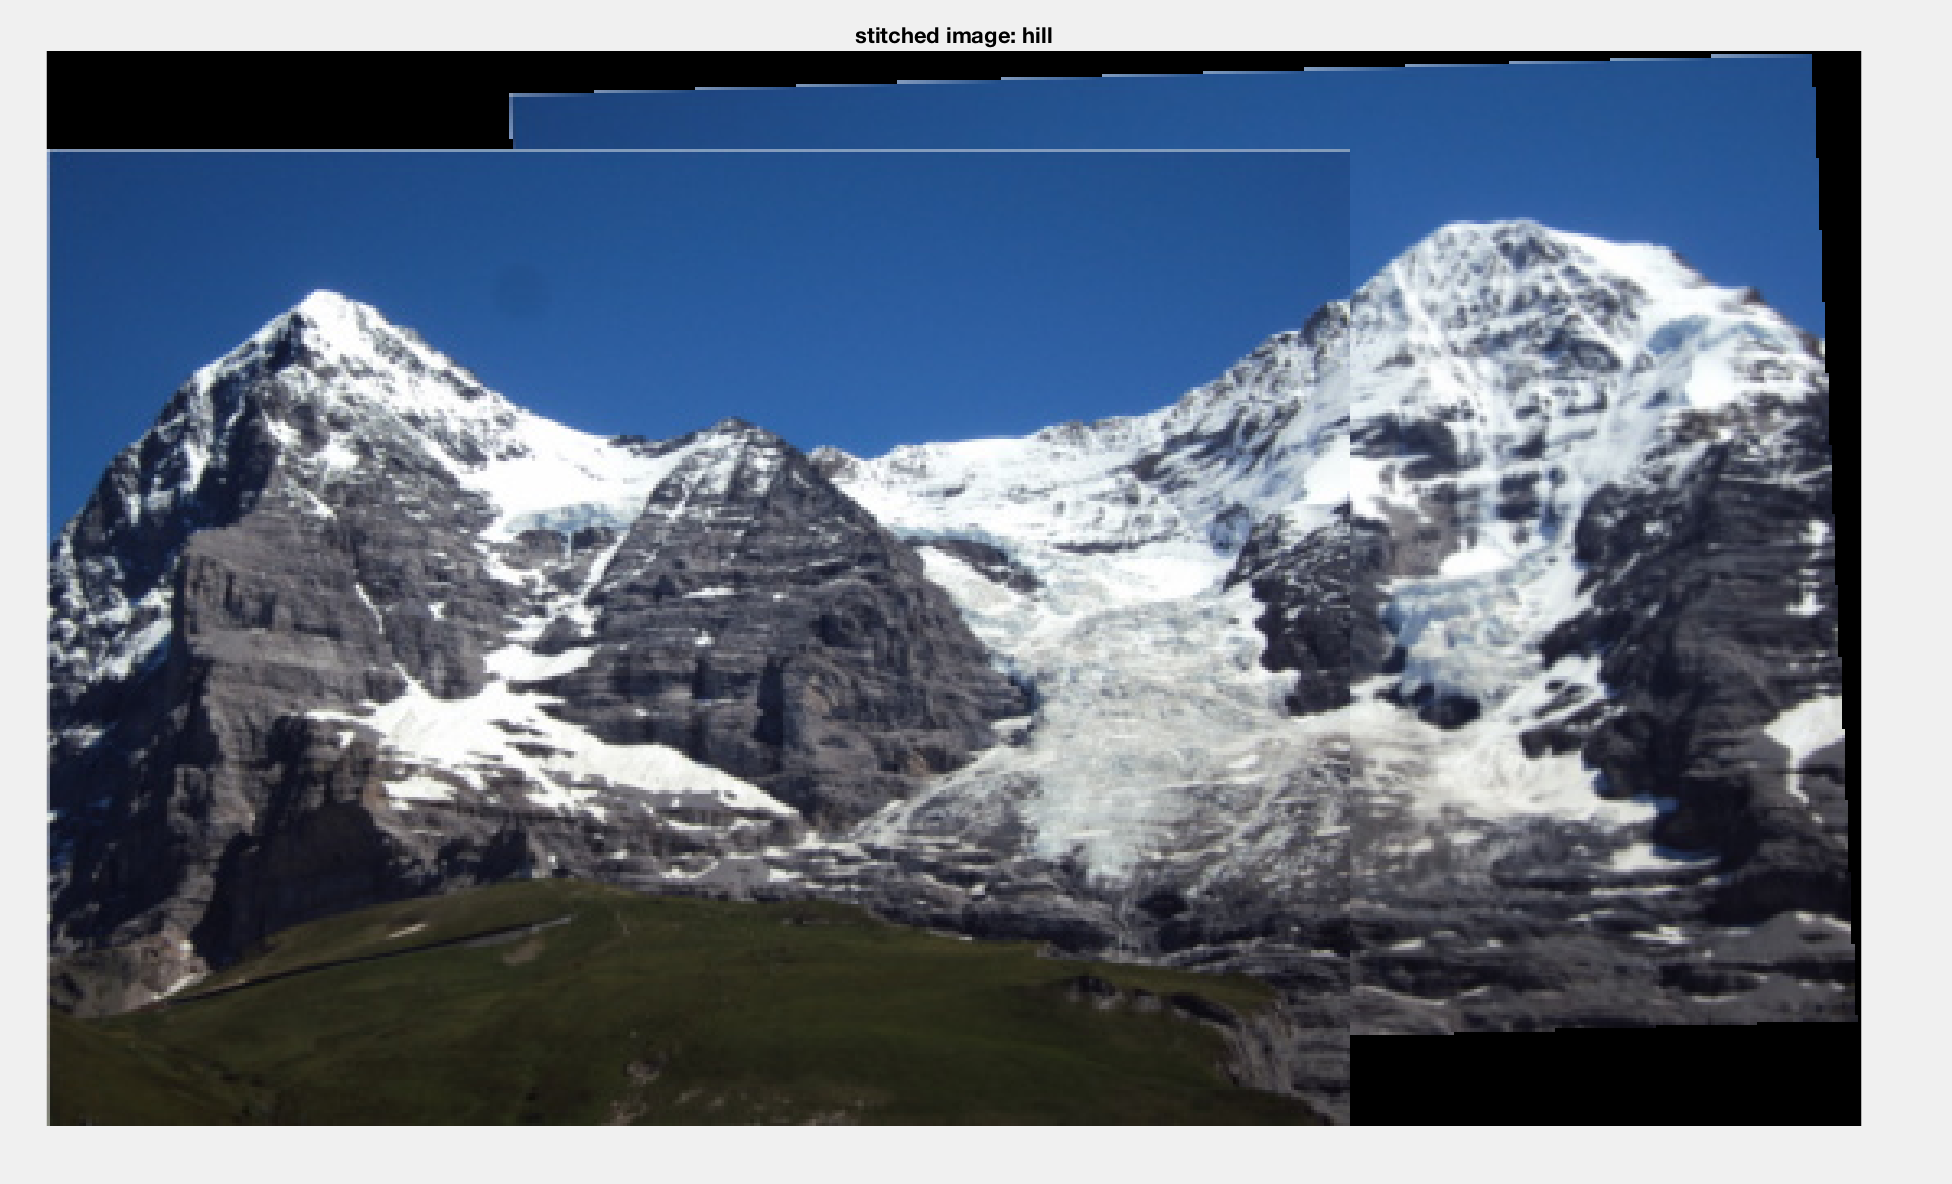
\includegraphics[width=0.95\linewidth]{./stich/hill.jpg} 
\caption{\label{fig:dummy} With Affine Transformation: Hill}
\end{figure}

\begin{figure}[h]
\centering
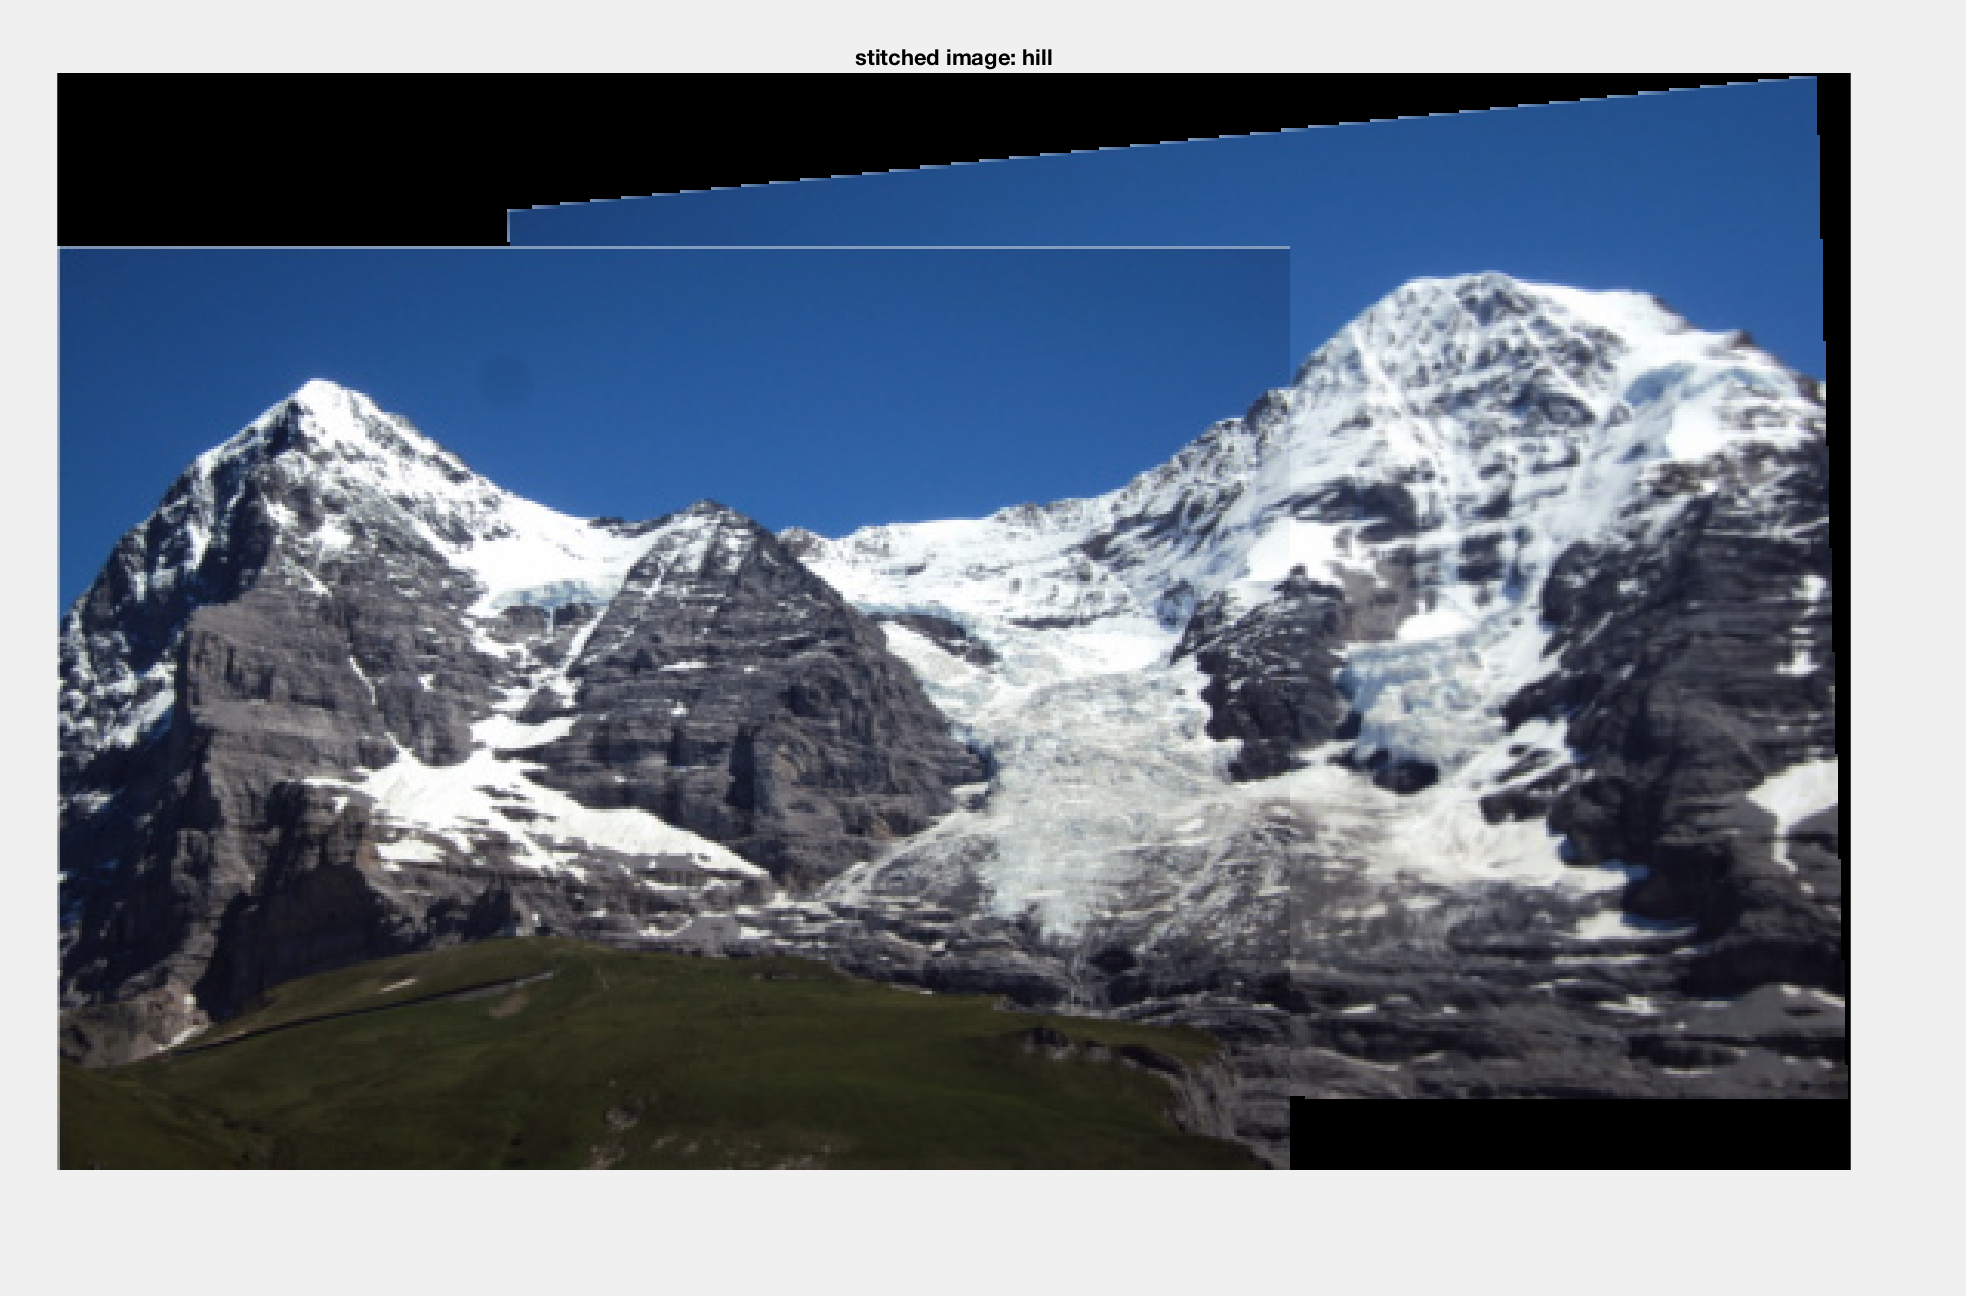
\includegraphics[width=0.95\linewidth]{./stich/Hhill.jpg} 
\caption{\label{fig:dummy} With homography transformation: Hill}
\end{figure}

\begin{figure}[h]
\centering
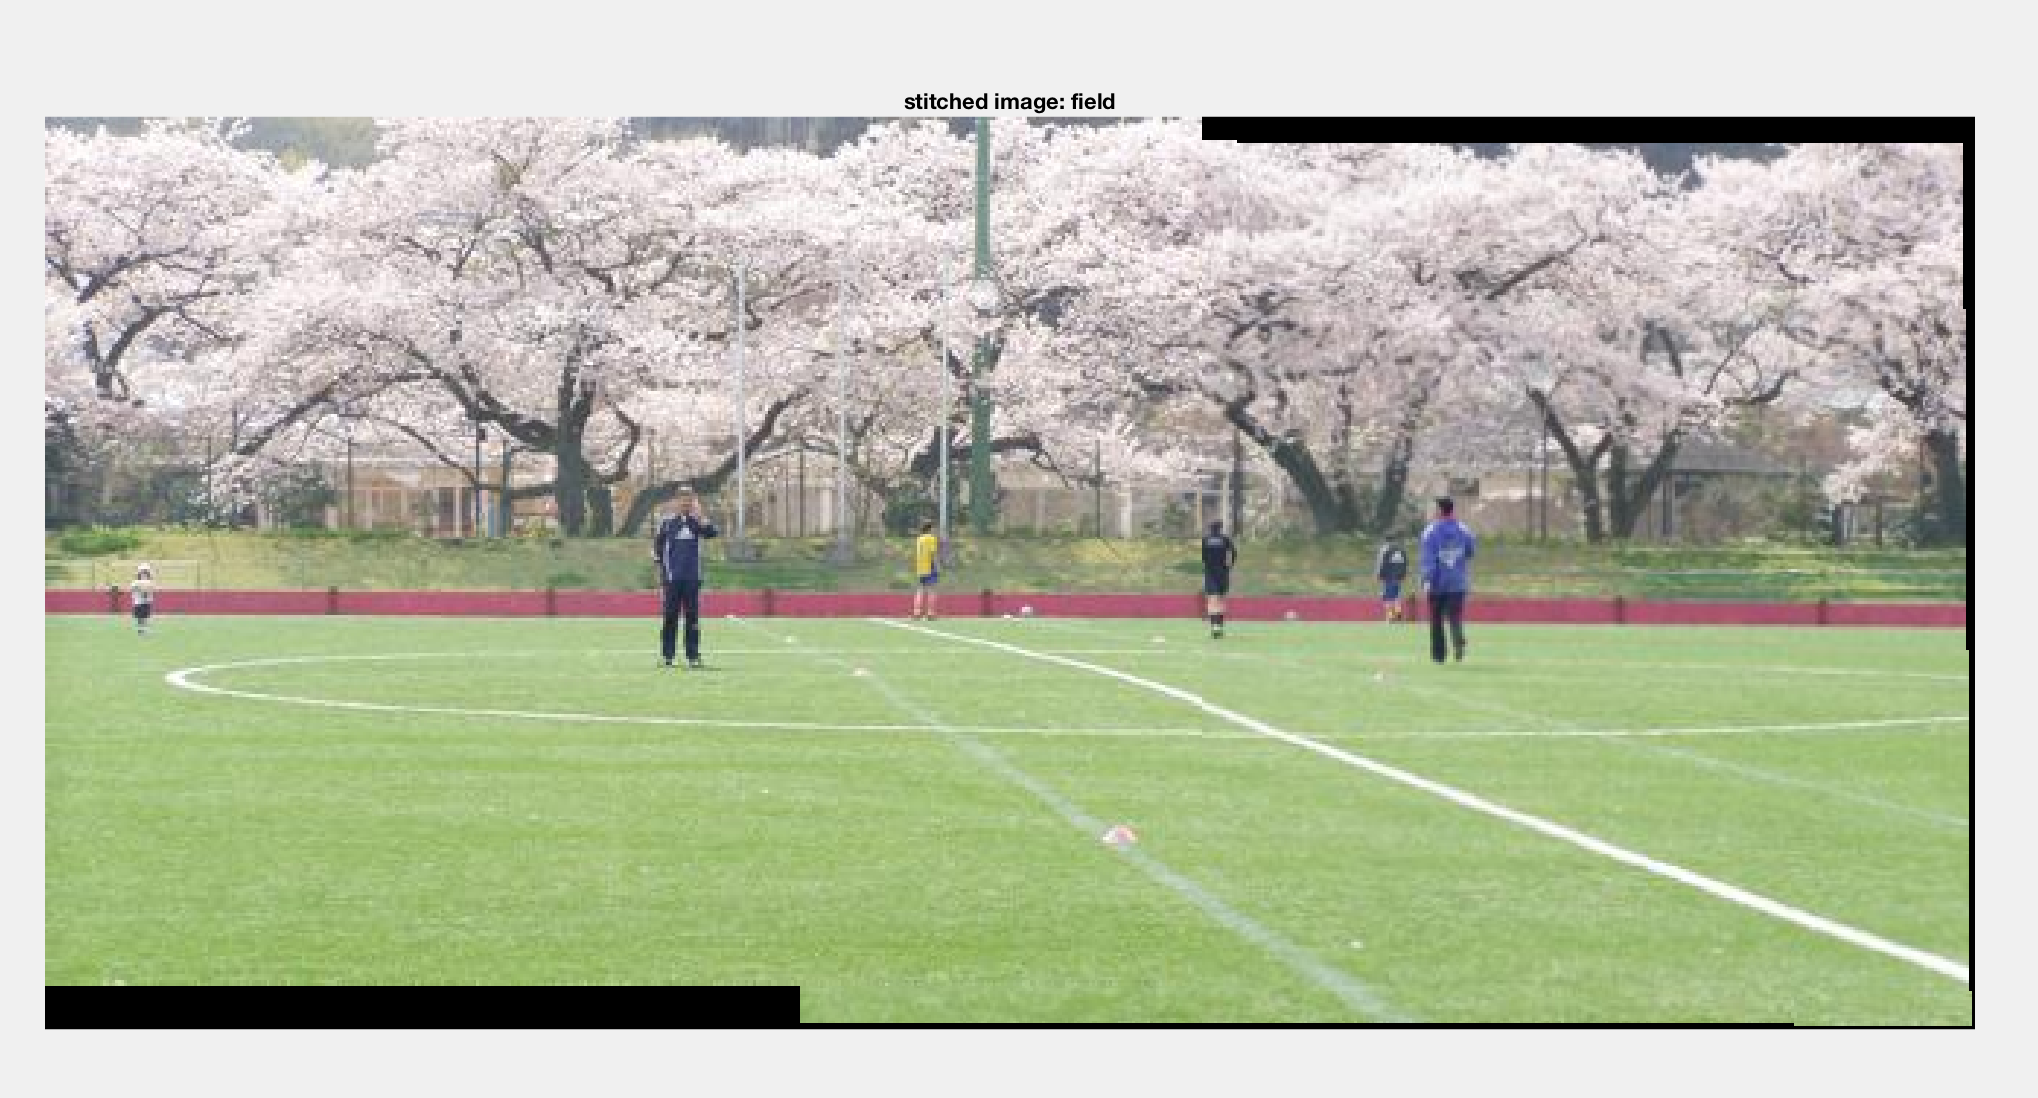
\includegraphics[width=0.95\linewidth]{./stich/field.jpg} 
\caption{\label{fig:dummy} With Affine Transformation: Field}
\end{figure}


\begin{figure}[h]
\centering
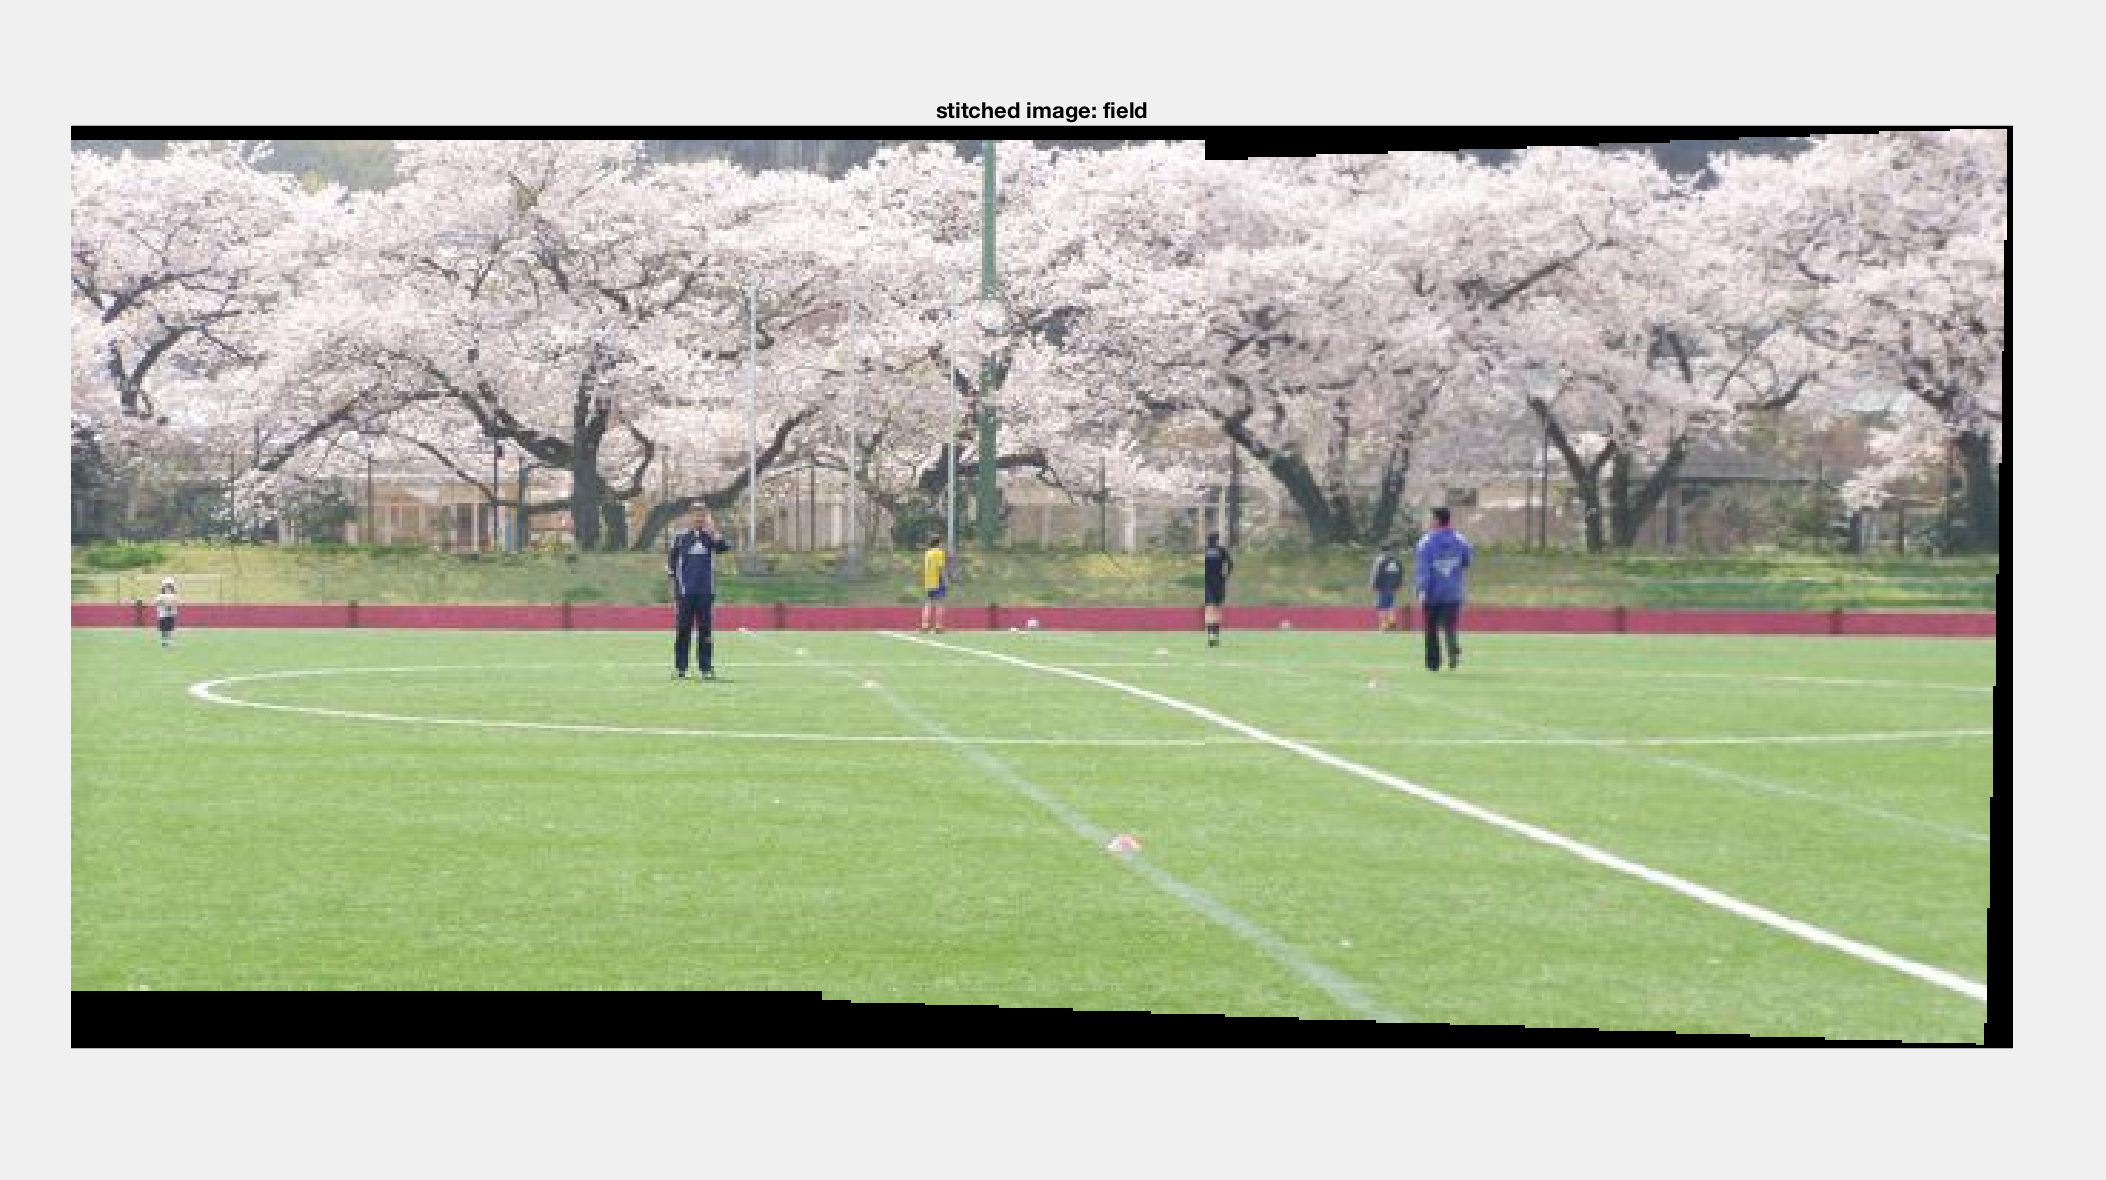
\includegraphics[width=0.95\linewidth]{./stich/Hfield.jpg} 
\caption{\label{fig:dummy} With homography transformation: Field}
\end{figure}

\begin{figure}[h]
\centering
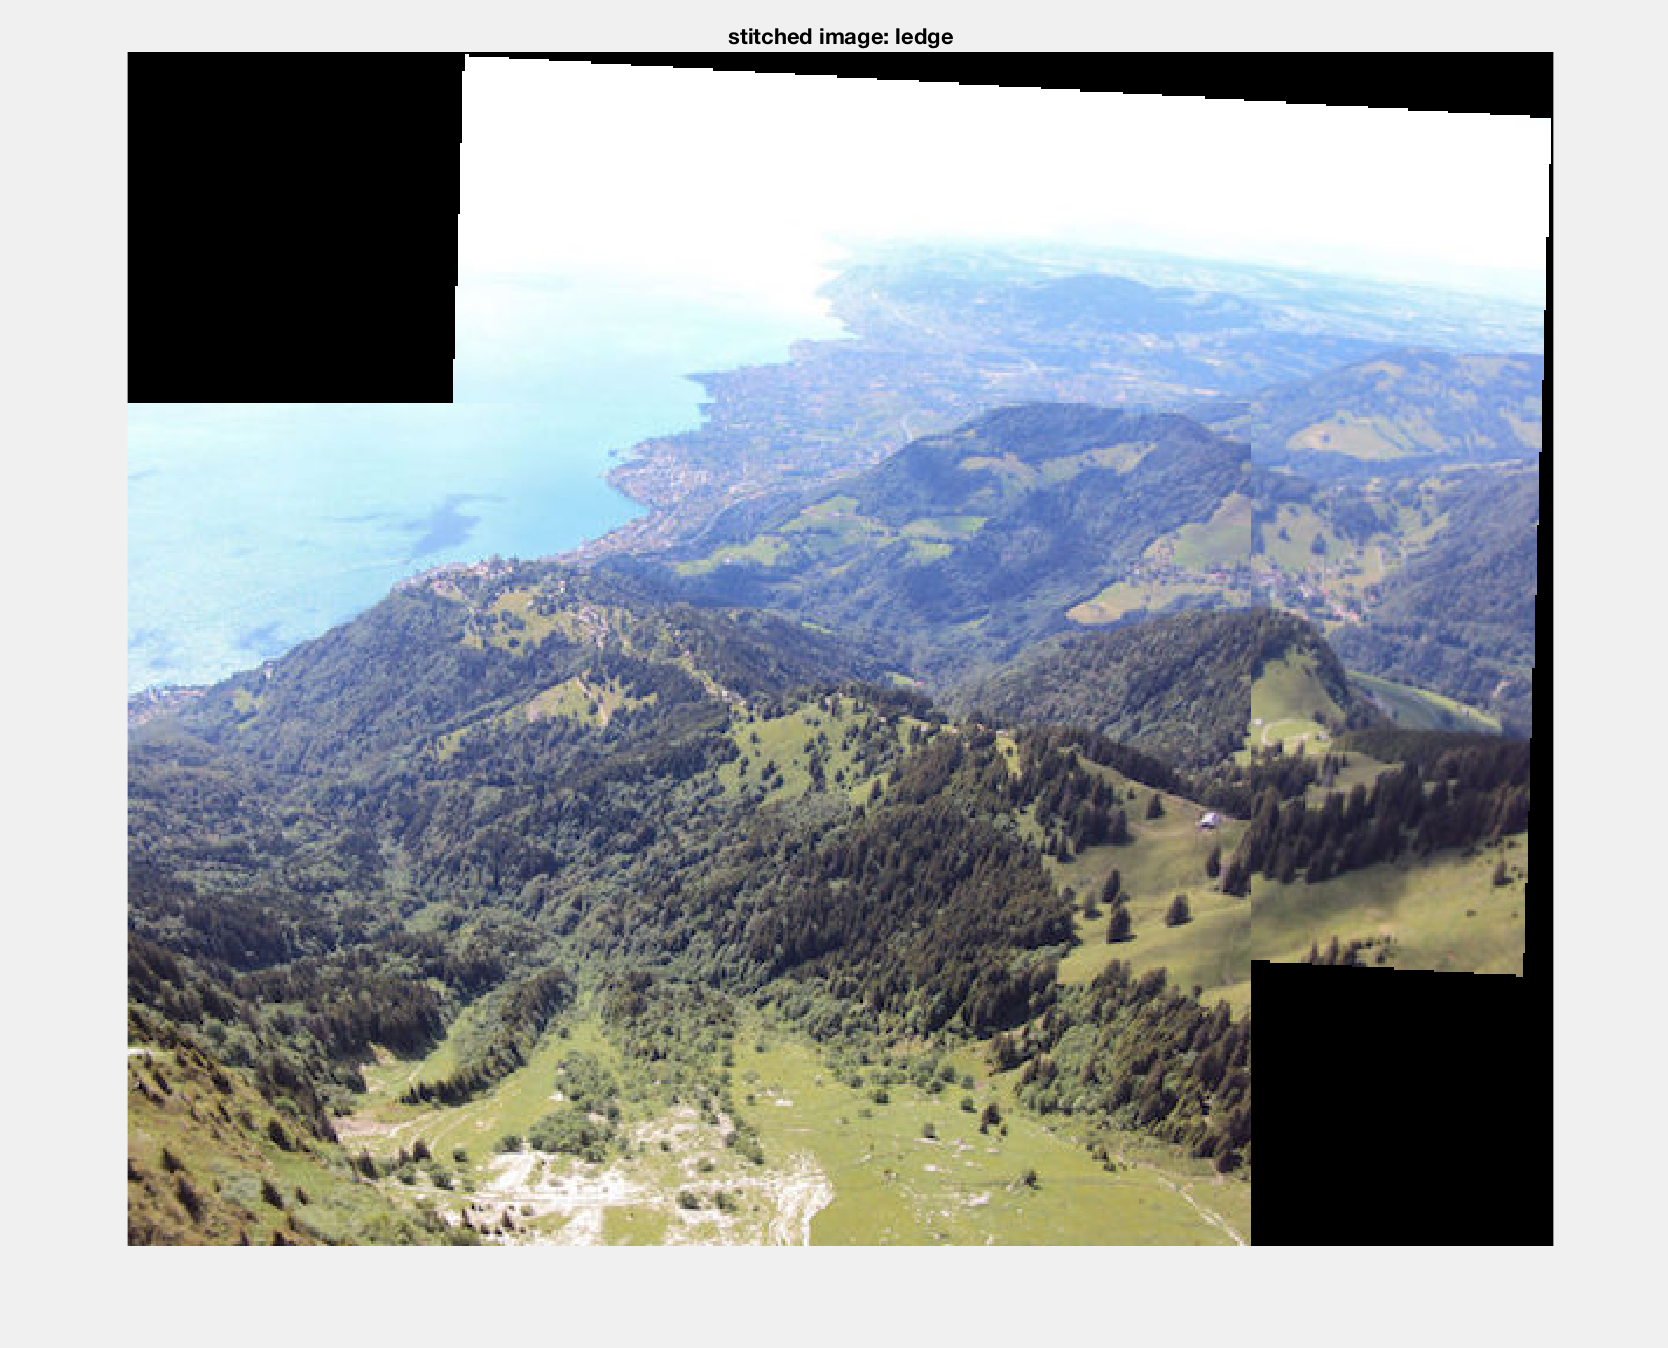
\includegraphics[width=0.95\linewidth]{./stich/ledge.jpg} 
\caption{\label{fig:dummy} With Affine Transformation: Ledge}
\end{figure}

\begin{figure}[h]
\centering
\includegraphics[width=0.95\linewidth]{./stich/Hledge.jpg} 
\caption{\label{fig:dummy}  With homography transformation: Ledge}
\end{figure}

\begin{figure}[h]
\centering
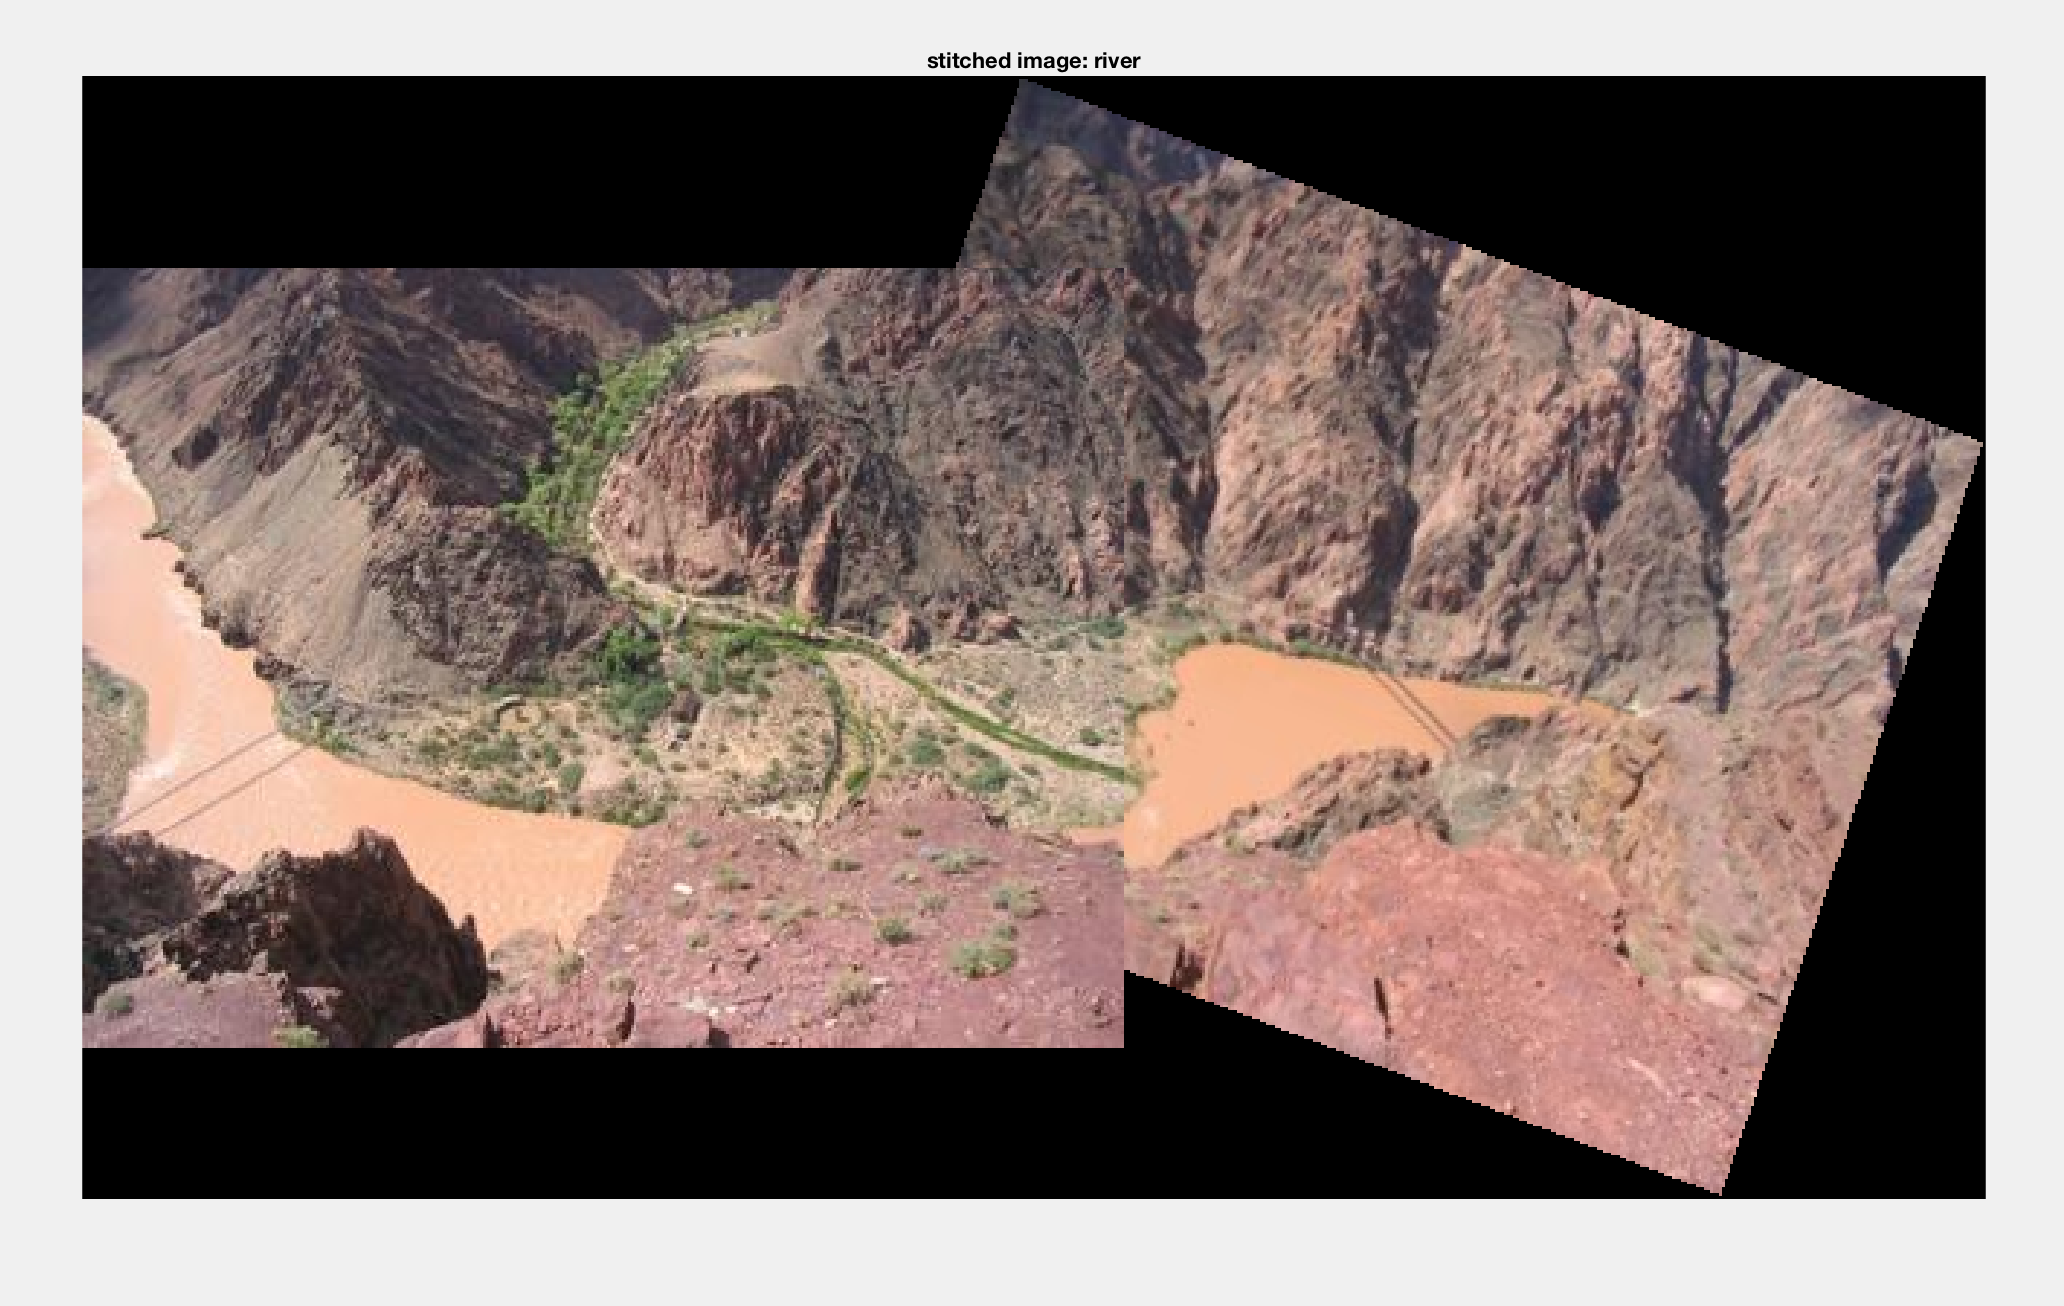
\includegraphics[width=0.95\linewidth]{./stich/river.jpg} 
\caption{\label{fig:dummy} With Affine Transformation: River}
\end{figure}

\begin{figure}[h]
\centering
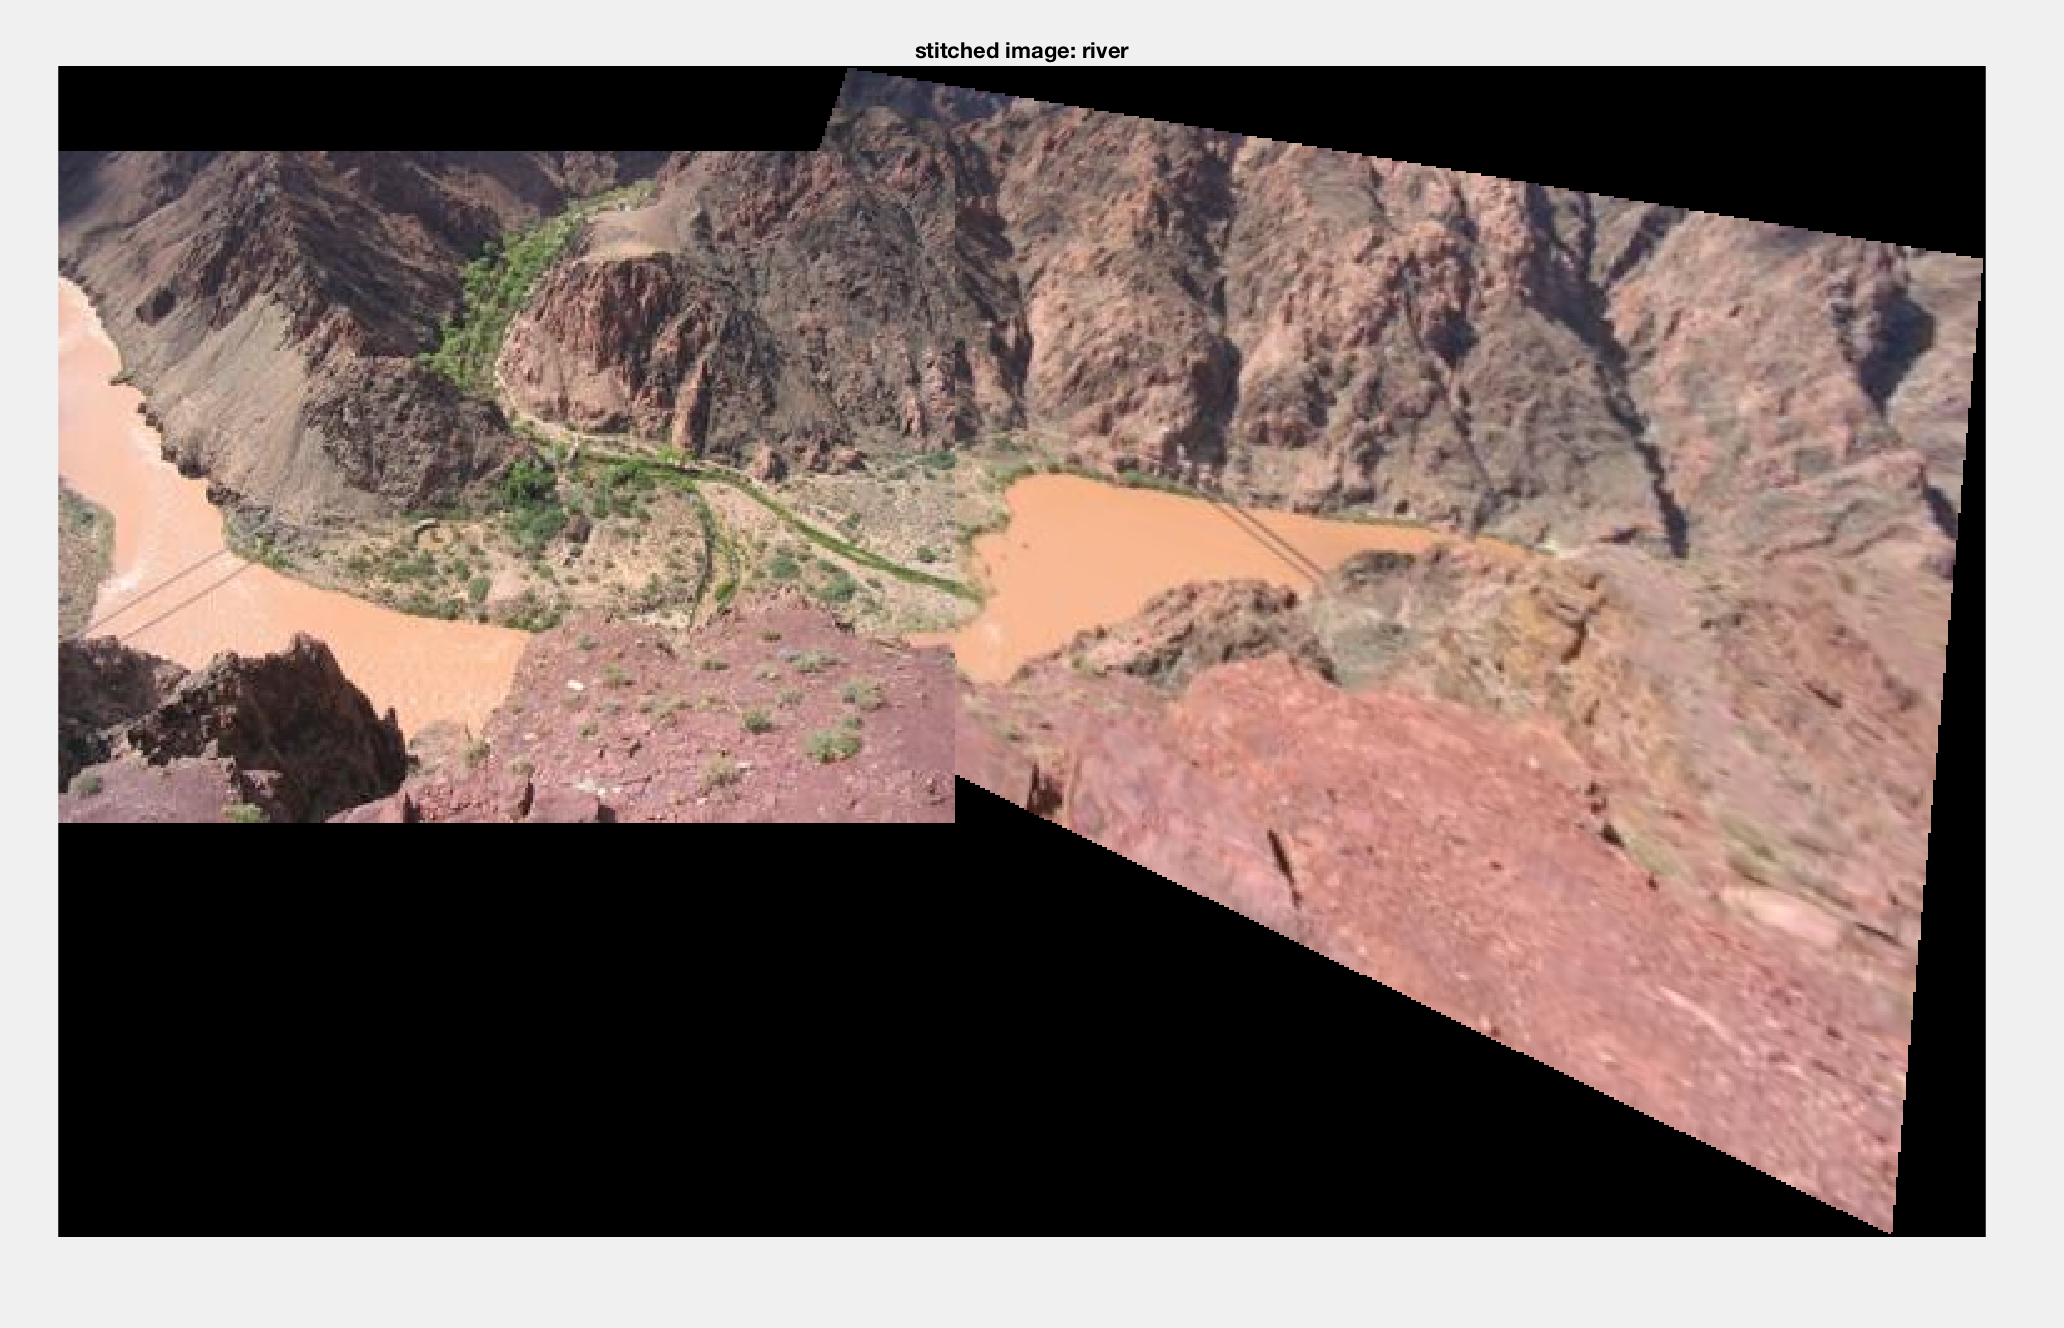
\includegraphics[width=0.95\linewidth]{./stich/Hriver.jpg} 
\caption{\label{fig:dummy}  With homography transformation: River}
\end{figure}   

\begin{figure}[h]
\centering
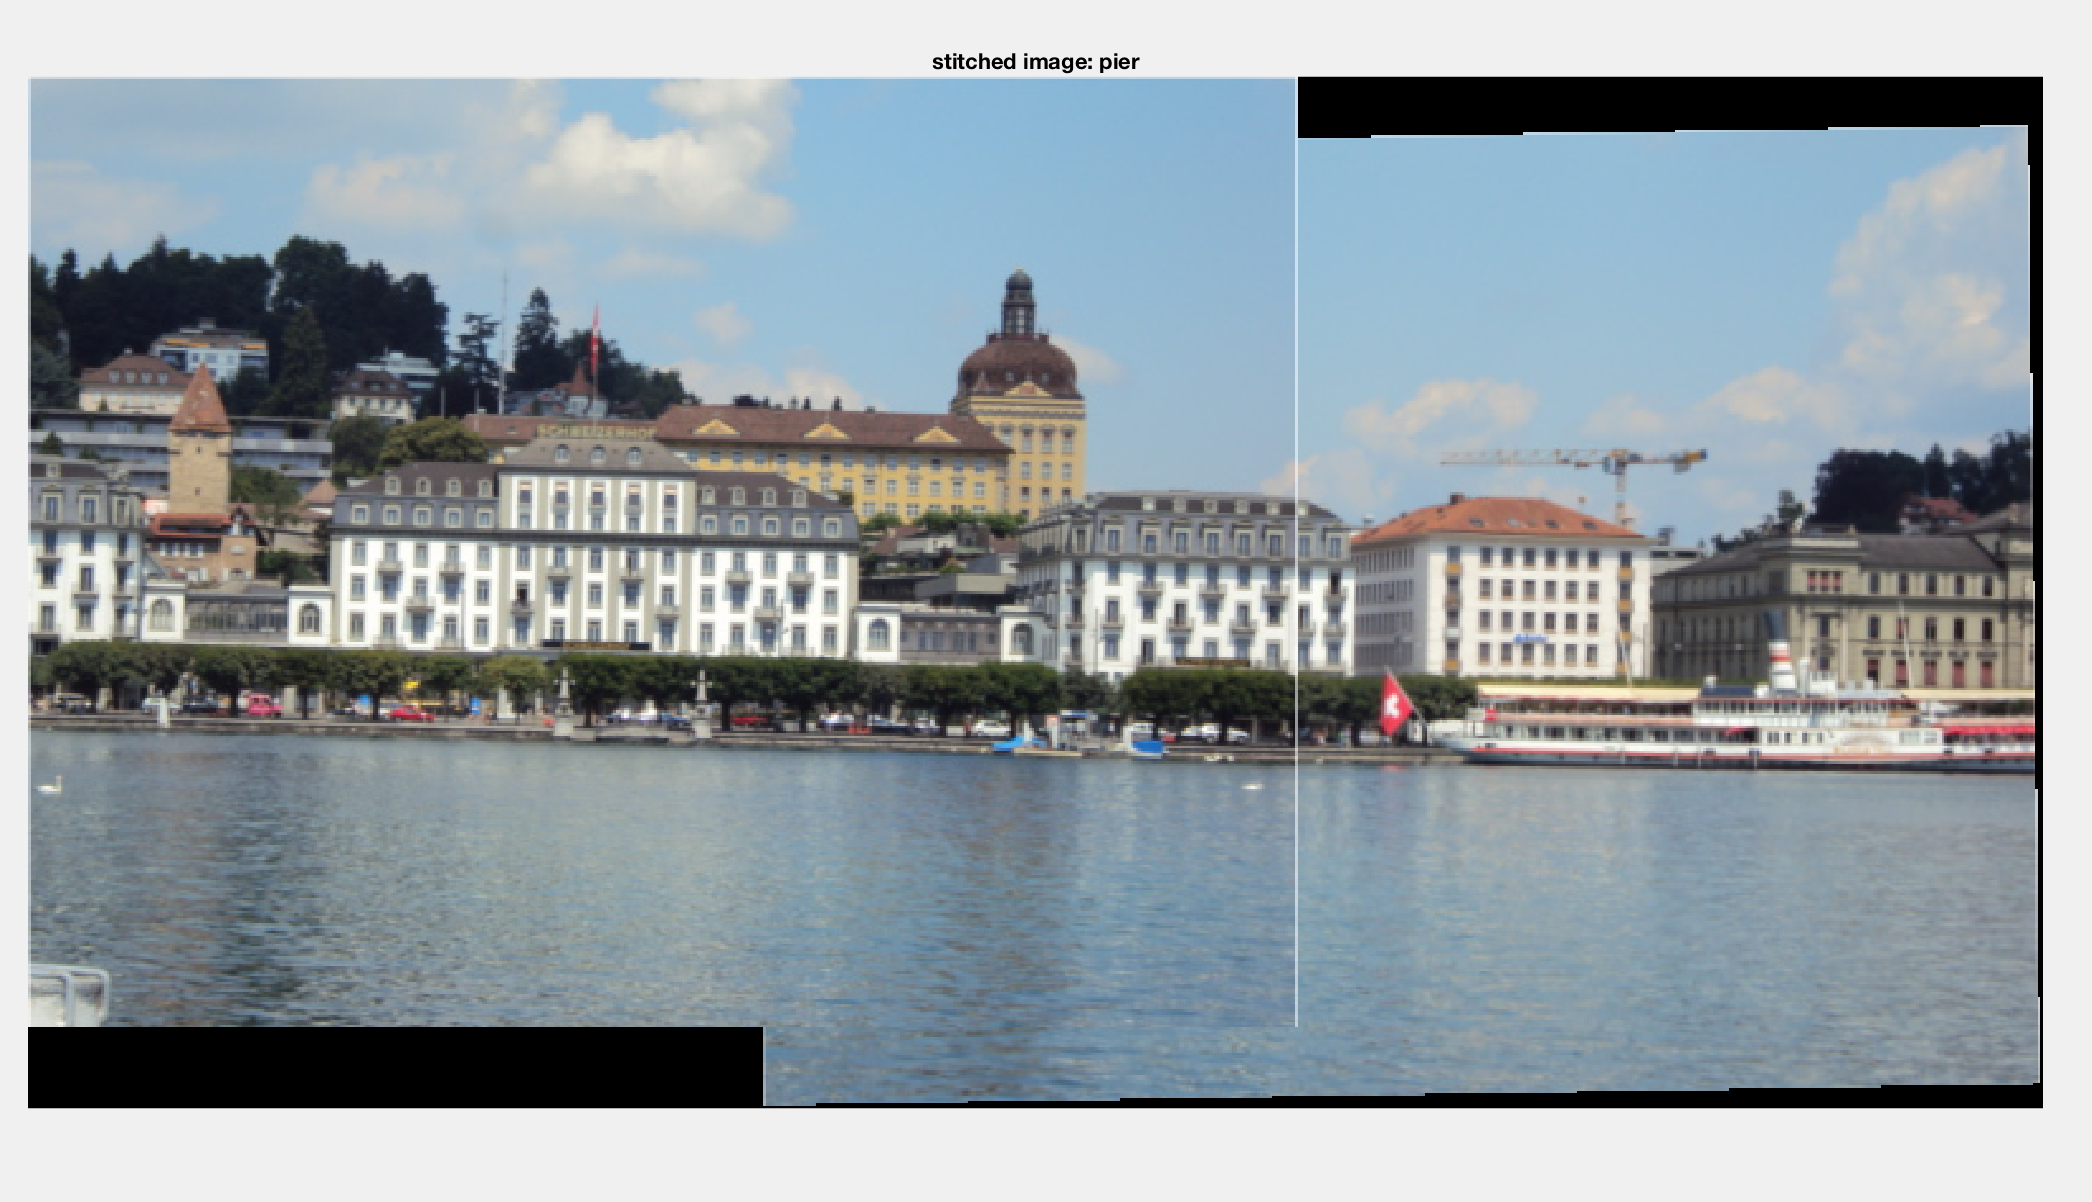
\includegraphics[width=0.95\linewidth]{./stich/pier.jpg} 
\caption{\label{fig:dummy} With Affine Transformation: Pier}
\end{figure}

\begin{figure}[h]
\centering
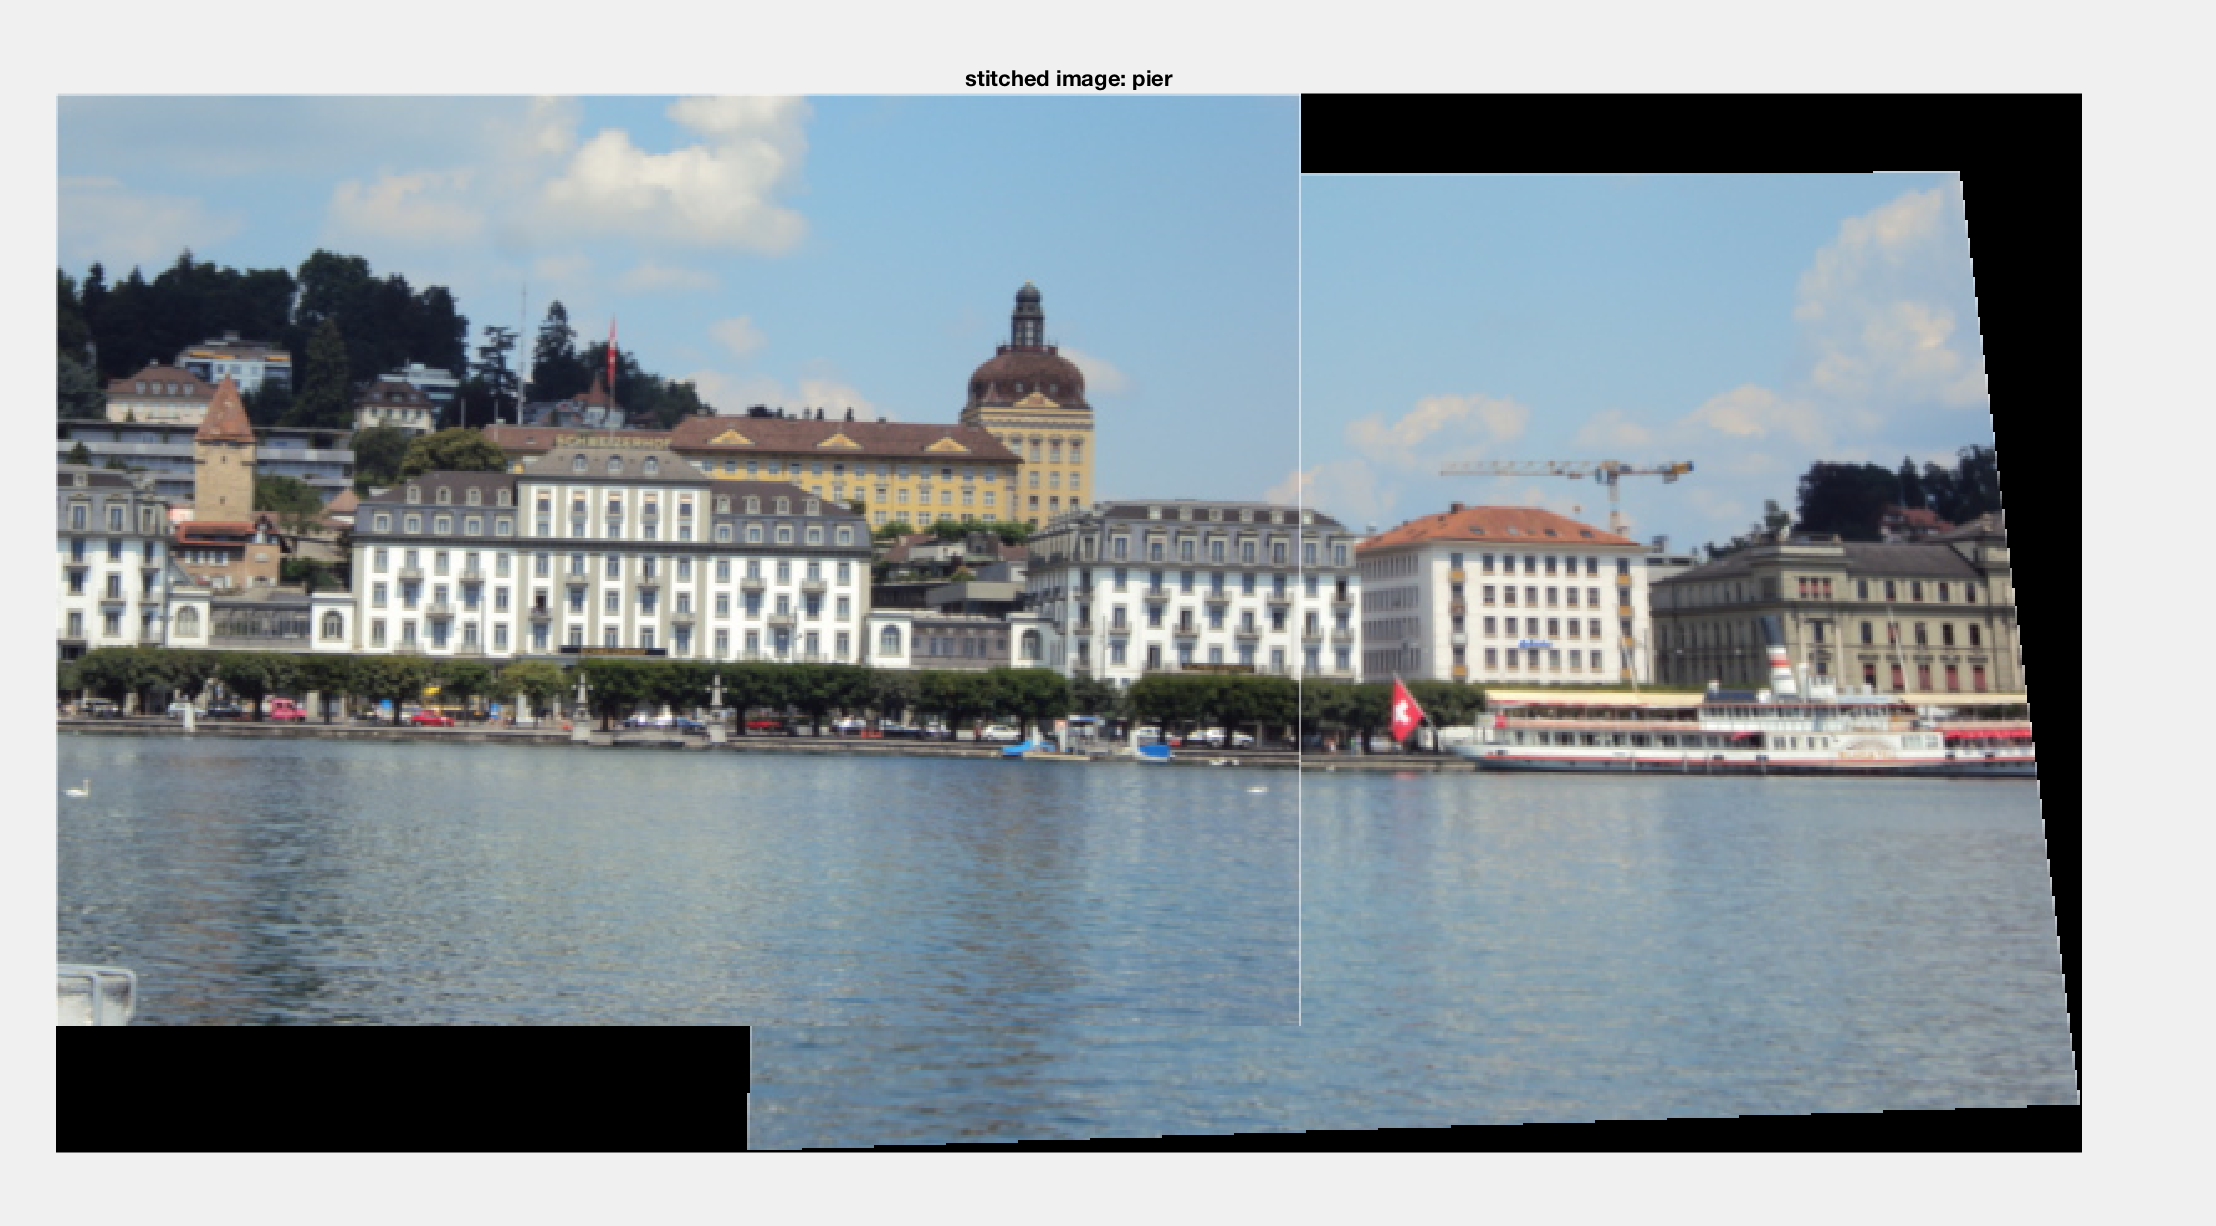
\includegraphics[width=0.95\linewidth]{./stich/Hpier.jpg} 
\caption{\label{fig:dummy}  With homography transformation:Pier}
\end{figure}

\begin{figure}[h]
\centering
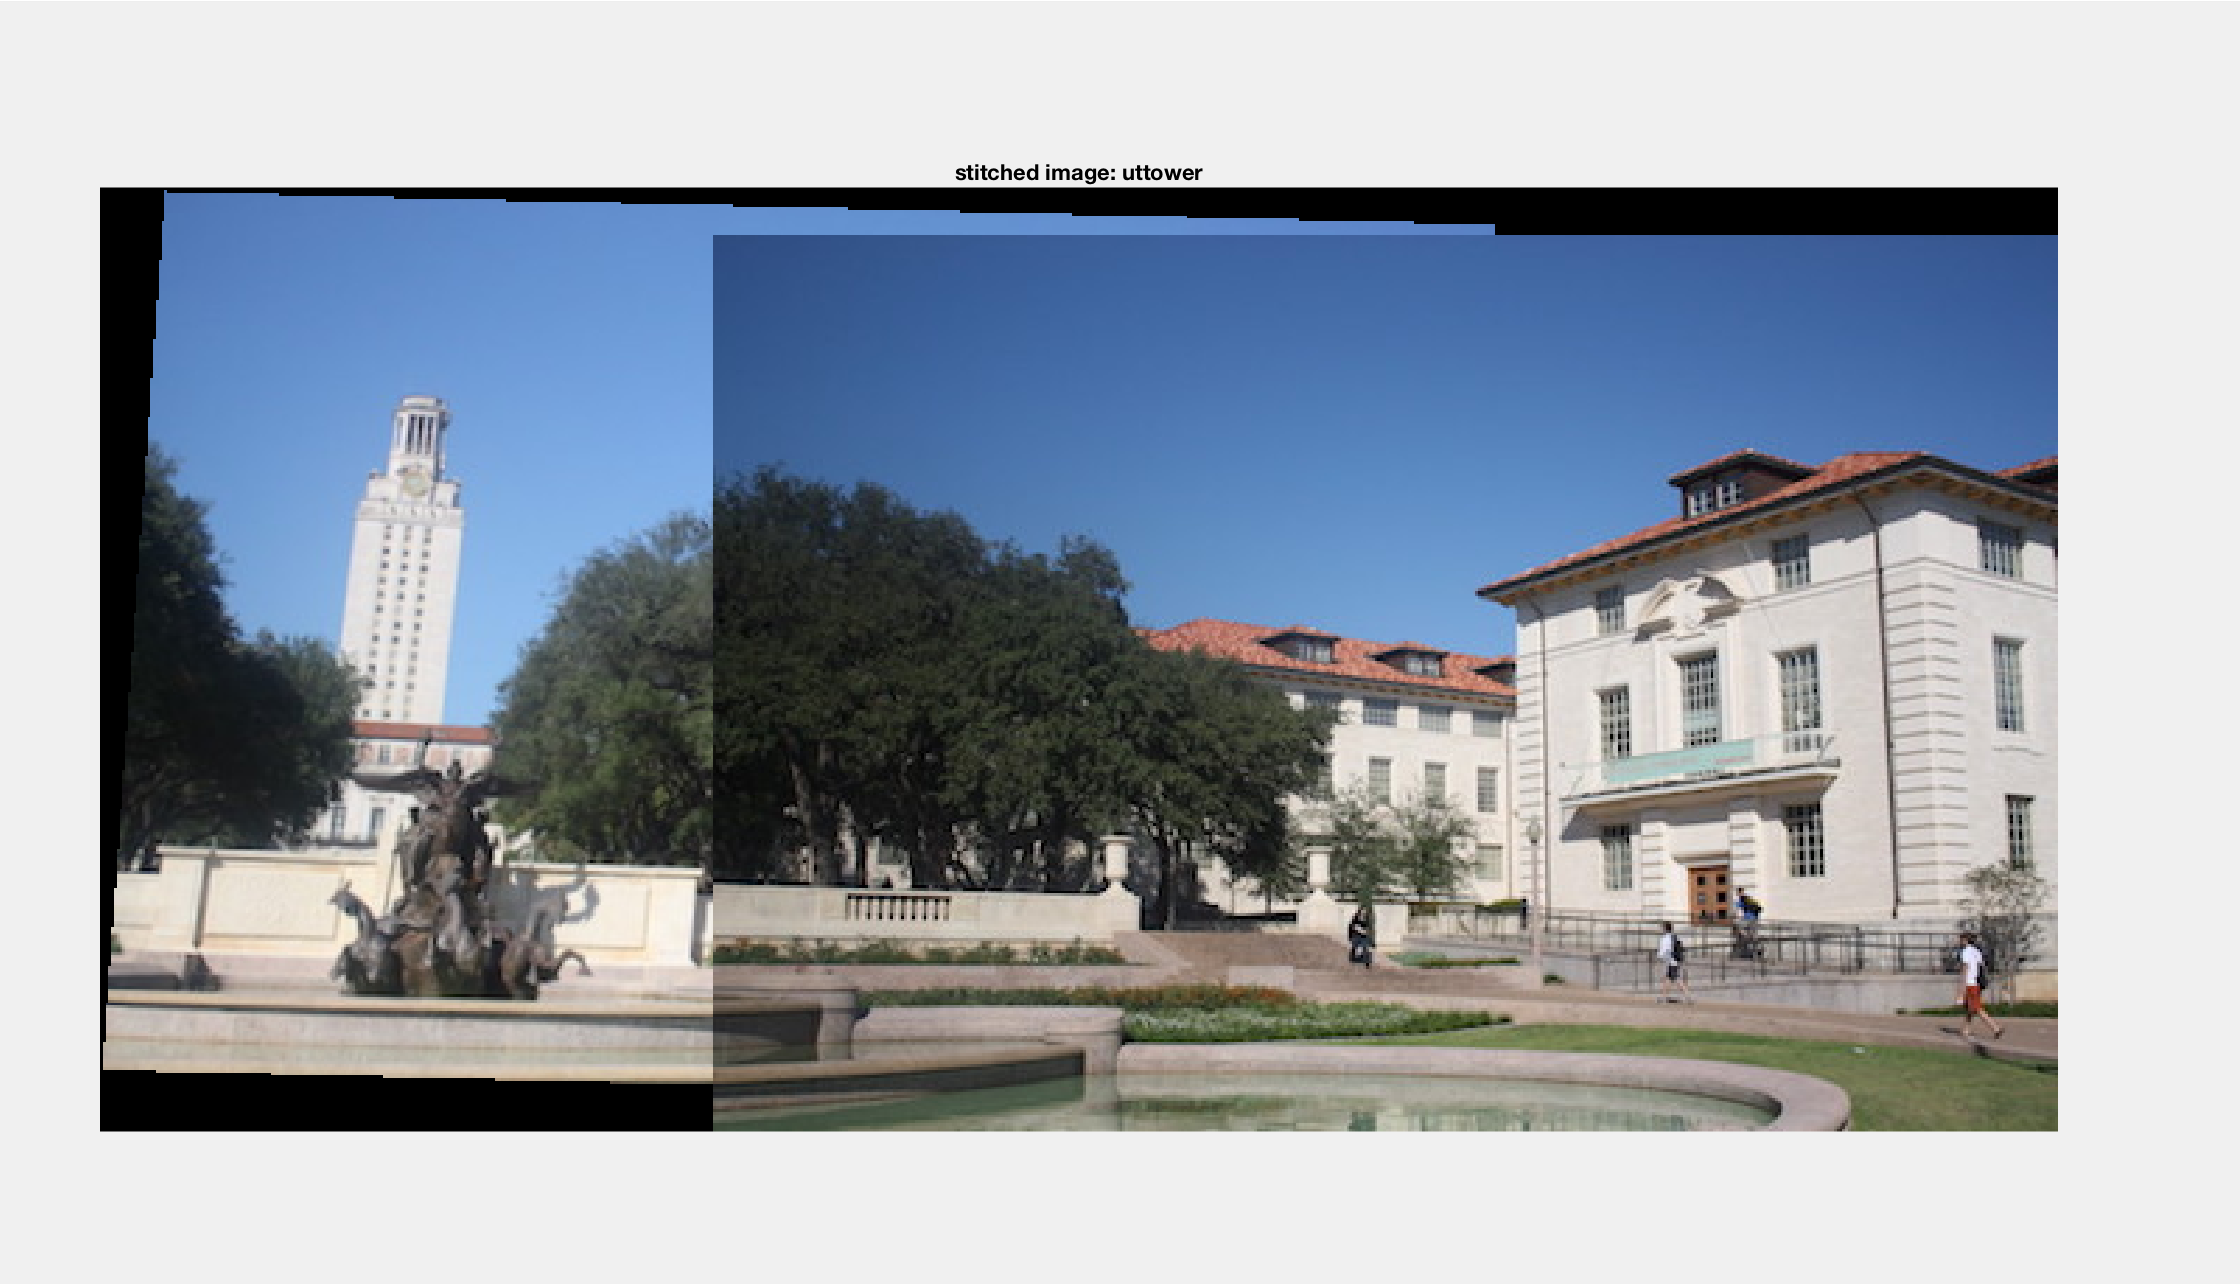
\includegraphics[width=0.95\linewidth]{./stich/tower.jpg} 
\caption{\label{fig:dummy} With Affine Transformation: Tower}
\end{figure}

\begin{figure}[h]
\centering
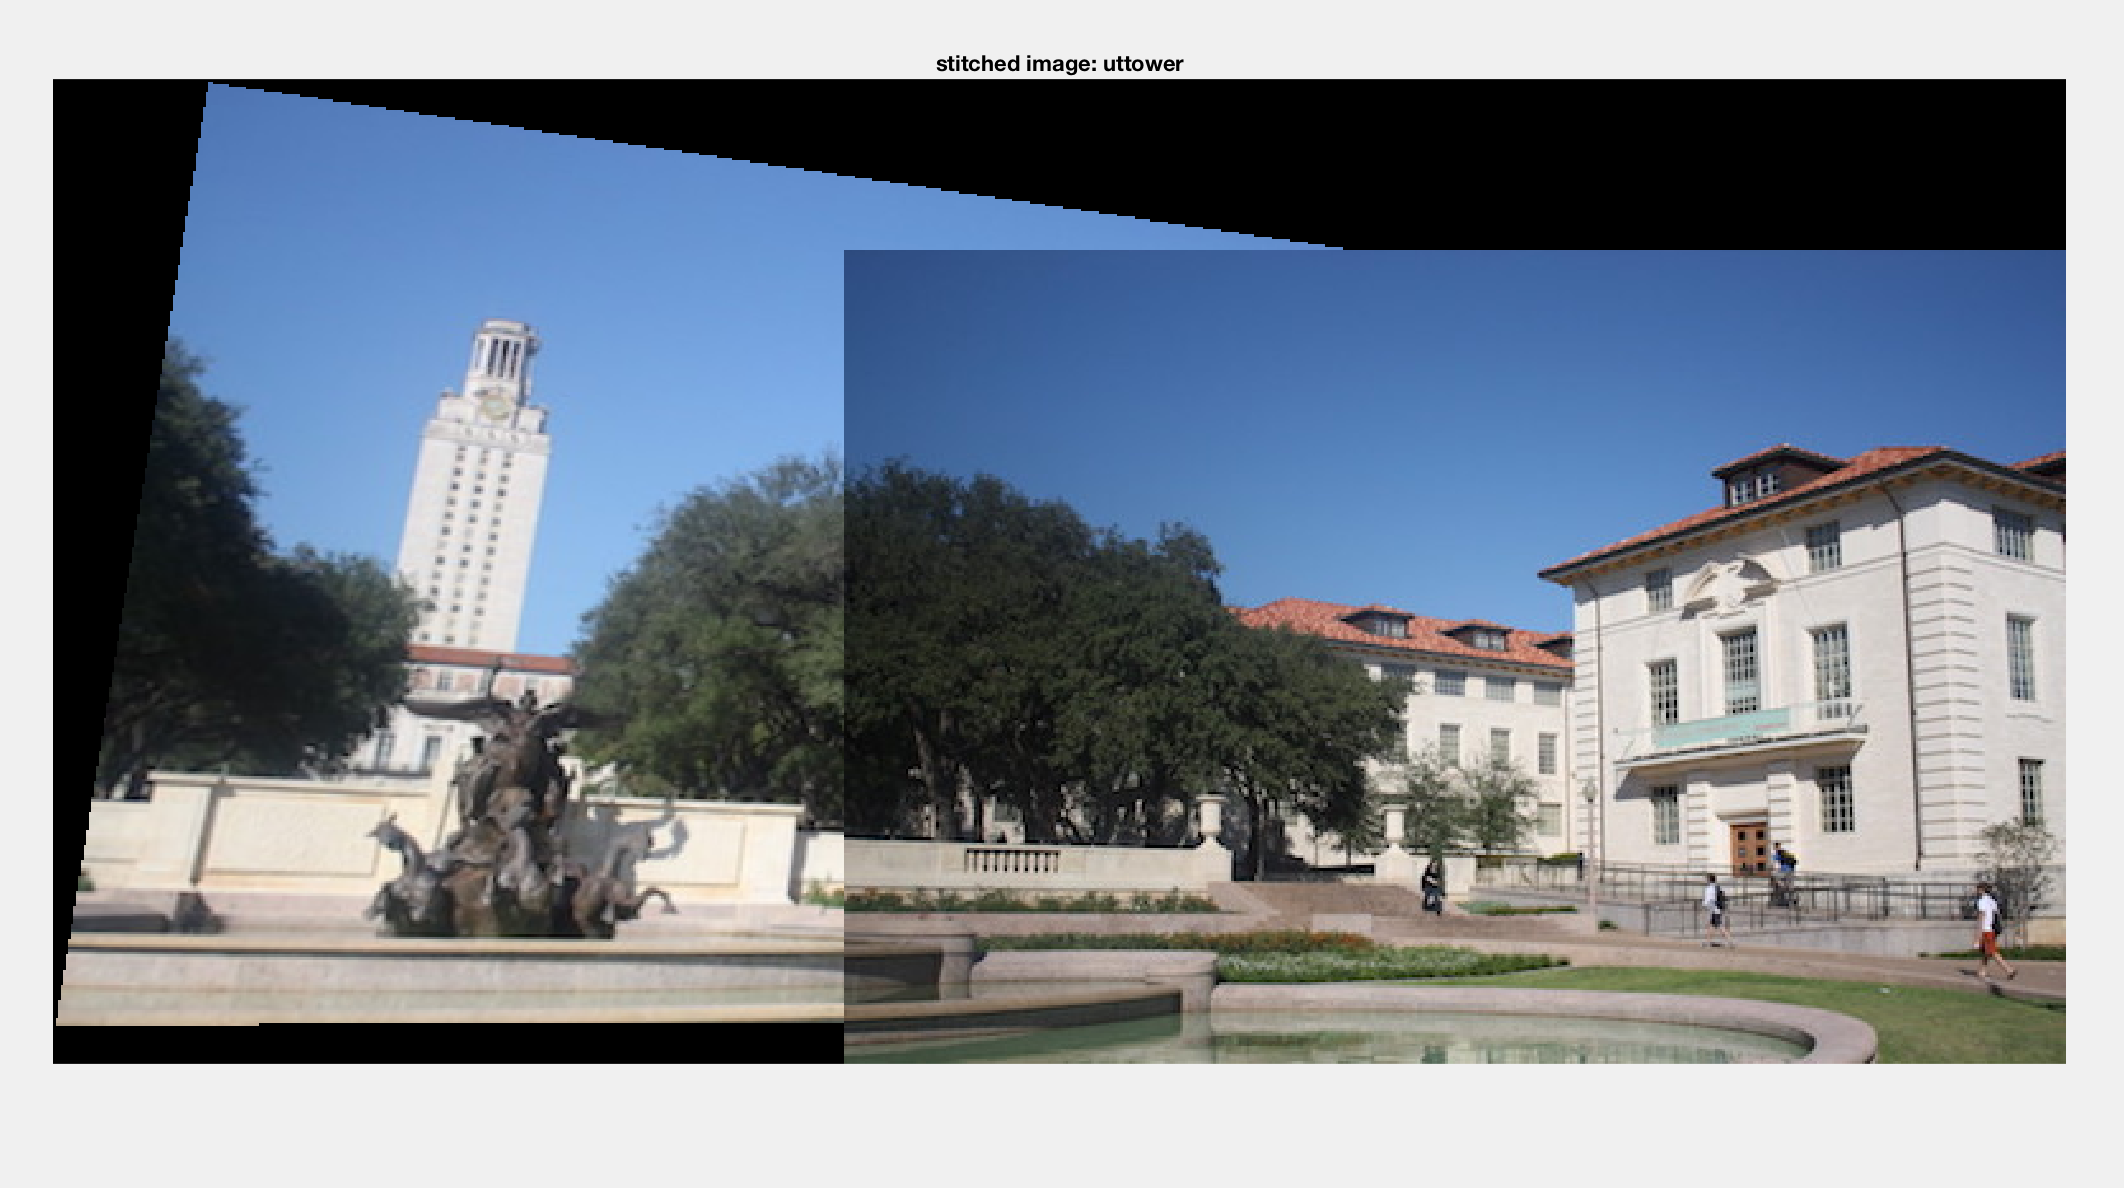
\includegraphics[width=0.95\linewidth]{./stich/Htower.jpg} 
\caption{\label{fig:dummy} With homography transformation: Tower}
\end{figure}

\begin{figure}[h]
\centering
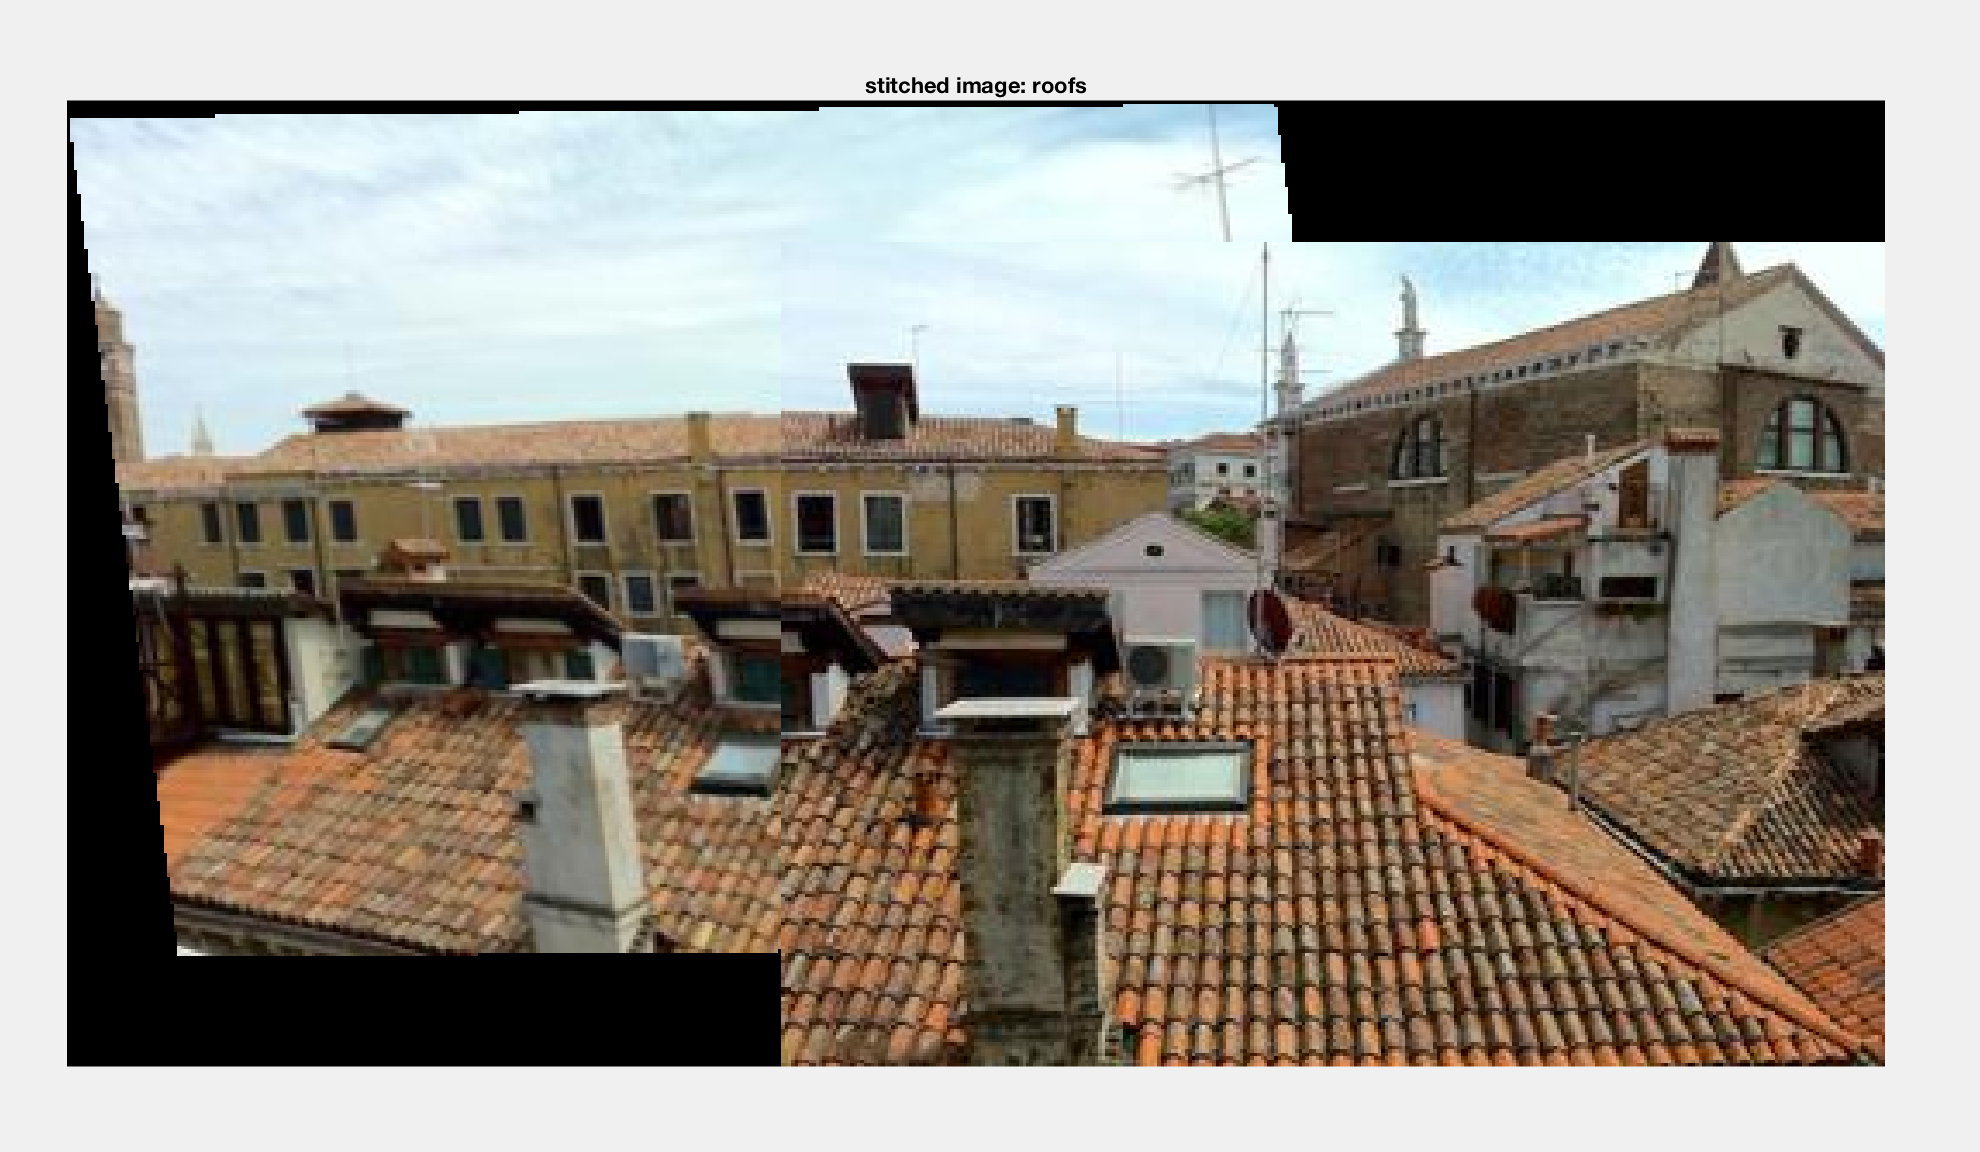
\includegraphics[width=0.95\linewidth]{./stich/roofs.jpg} 
\caption{\label{fig:dummy} With Affine Transformation: Roof}
\end{figure}


\begin{figure}[h]
\centering
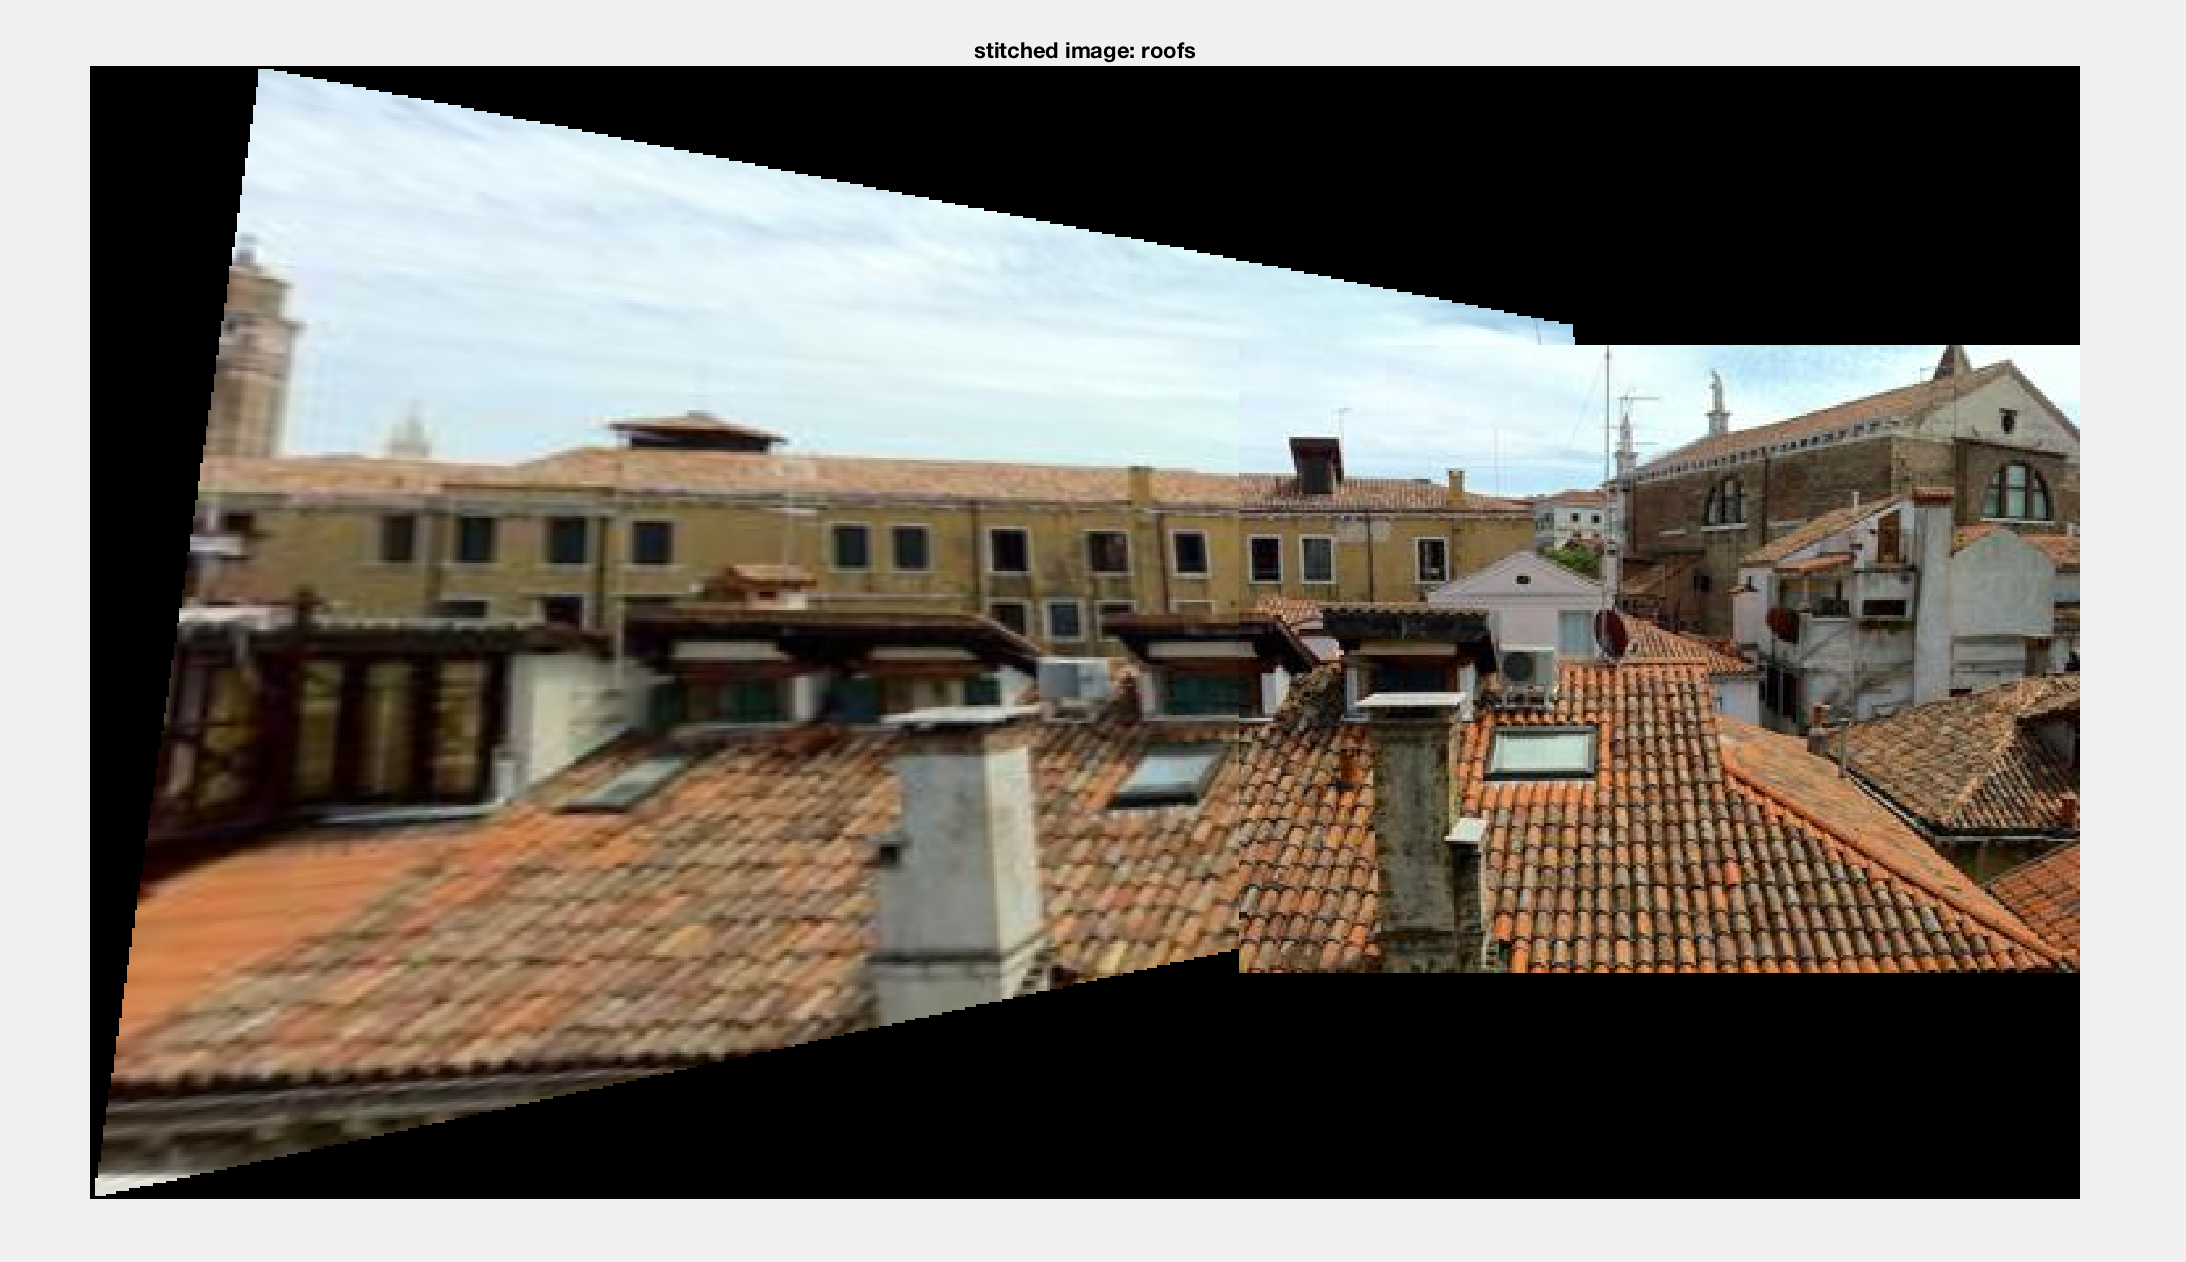
\includegraphics[width=0.95\linewidth]{./stich/Hroofs.jpg} 
\caption{\label{fig:dummy} With homography transformation: Roof}
\end{figure}

\begin{figure}[h]
\centering
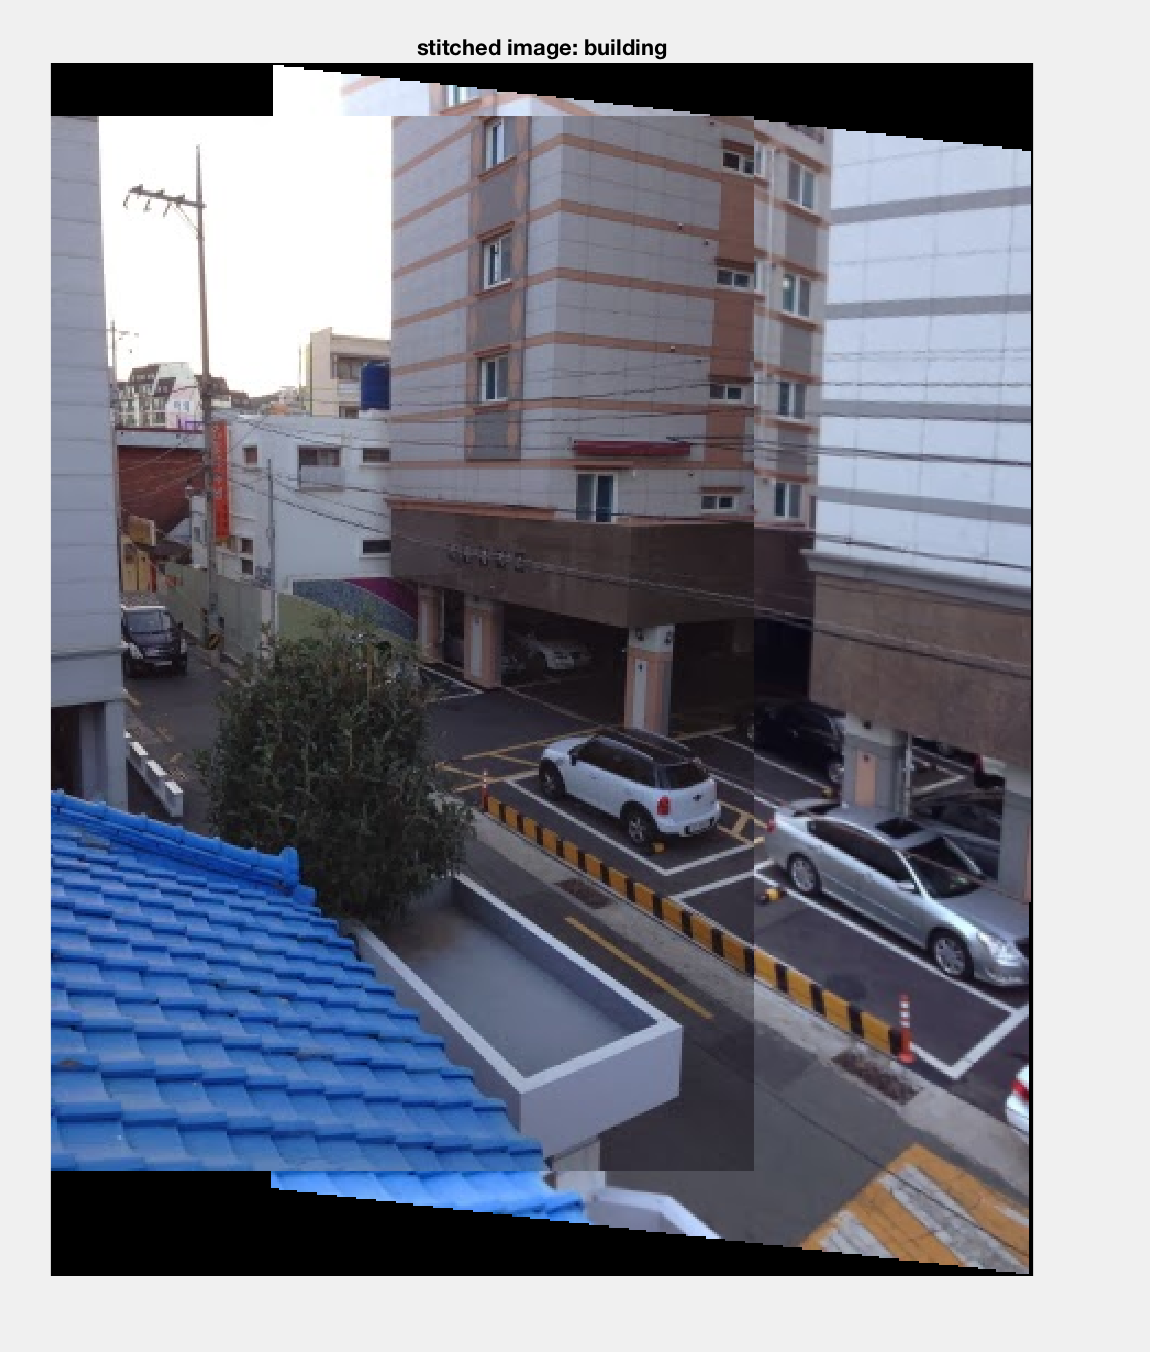
\includegraphics[width=0.95\linewidth]{./stich/building.jpg} 
\caption{\label{fig:dummy} With Affine Transformation: Building}
\end{figure}

\begin{figure}[h]
\centering
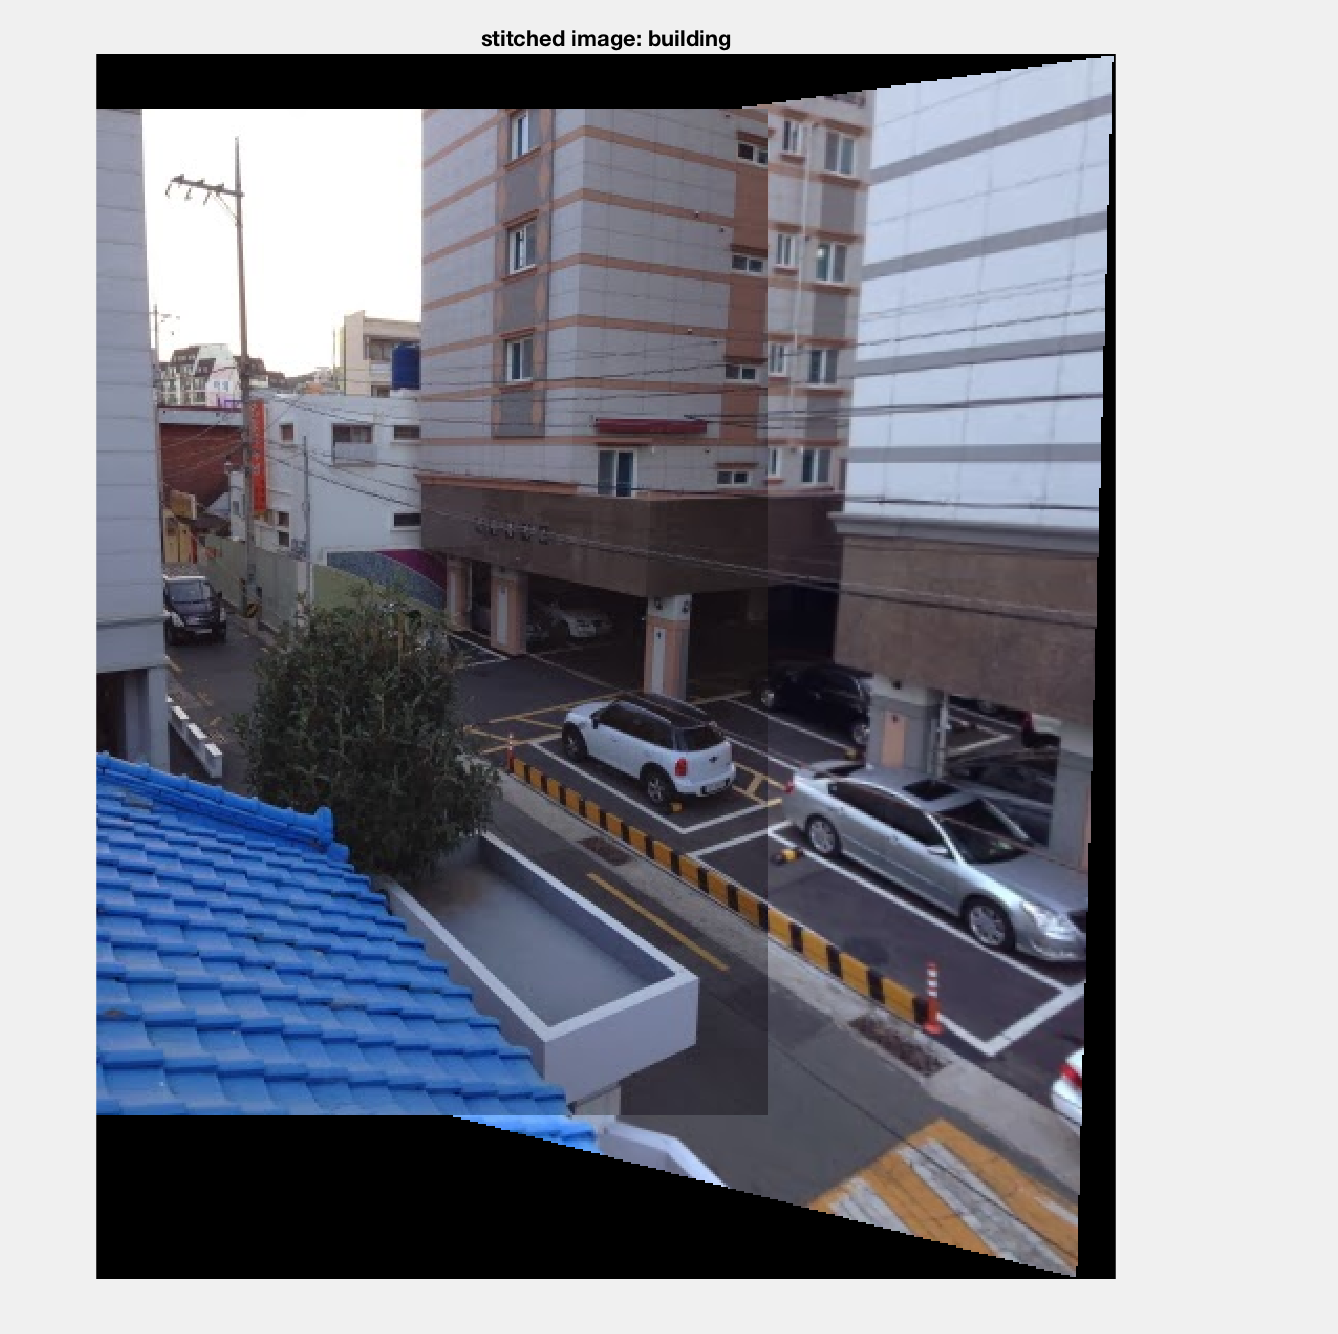
\includegraphics[width=0.95\linewidth]{./stich/Hbuilding.jpg} 
\caption{\label{fig:dummy}  With homography transformation: Building}
\end{figure}
\newpage


\end{document}
